\documentclass[fleqn,10pt]{wlscirep}
\usepackage[utf8]{inputenc}
\usepackage[T1]{fontenc}
\usepackage{array}
\usepackage{algorithm}
\usepackage{algpseudocode}

\newcolumntype{L}[1]{>{\raggedright\arraybackslash}p{#1}}
\DeclareRobustCommand{\code}[1]{\path{#1}}
\newcommand{\RankOf}{\operatorname{rank\_of}}
\newcommand{\Encode}{\operatorname{encode}}
\newcommand{\Decode}{\operatorname{decode}}
\newcommand{\Tokenize}{\operatorname{tokenize}}
\newcommand{\Detokenize}{\operatorname{detokenize}}
\newcommand{\NextLogits}{\operatorname{next\_logits}}


\title{RankCloak: Hiding Synthetic Cryptographic Artifacts in Plain English with Language Models}
%\title{RankCloak: Measuring Hidden Synthetic Cryptographic Artifacts in Language Model Text}



\author[1,*]{Alexander V. Mantzaris}
\affil[1]{School of Data, Mathematical, and Statistical Sciences, University of Central Florida, Orlando, FL, United States of America}
\affil[*]{Correspondence: alexander.mantzaris@ucf.edu}


\keywords{steganography, large language models, rank transcoding, synthetic payloads, exact-copy recovery}


\begin{abstract}
Large language model (LLM) rank-transcoding steganography can contain a hidden payload as generated natural text by converting payload symbols into next-token ranks and reproducing those ranks under a cover prompt. We introduce RankCloak, a reproducible methodology for hiding synthetic cryptographic artifacts, including hashes, nonces, random hex strings, UUID-like values, and ciphertext-like text, inside plain English messages under exact-copy replay. RankCloak compares direct subword ranks with bounded ASCII-byte and hex-nibble encodings, and evaluates prompt-key generation, deterministic token filtering, segmented multi-cover messages, natural tails, and forced-span decoding. In the evaluated corpus, we analyze different cryptographic payloads and methodologies to produce natural appearing text which can be reversed. The methods explore segmented and non-segmented approaches to the cryptographic artifacts showing that the non-segmented is more robust. Direct subword encoding was compact but produced extreme rank outliers, whereas bounded encodings constrained rank pressure while increasing cover length. Segmented variants show that payload-bearing forced spans must be evaluated separately from full public messages because natural tails are visible cover text but carry no payload ranks. These results establish RankCloak as a practical methodology for hiding synthetic cryptographic artifacts in plain English.
\end{abstract}



\begin{document}

\flushbottom
\maketitle
\thispagestyle{empty}



\section*{Introduction}

Generative language models provide a new medium for text steganography because a prompt can define a next-token distribution and a topic direction in which generated text appears. In the recently proposed Calgacus algorithm rank-transcoding construction \cite{NorelliBronstein2025Calgacus}, a sender encodes a payload as a sequence of token ranks under one context (secret), generates cover text by selecting tokens at the corresponding ranks under a shared prompt context (key), and recovers the ranks by replaying the received token sequence with the same model and prompt configuration (same key prompt) \cite{NorelliBronstein2025Calgacus}. This mechanism connects classical work on covert channels, information-theoretic steganography, information hiding, and provably secure steganography \cite{Simmons1984Prisoners,Cachin1998InformationTheoretic,Hopper2002ProvablySecureSteganography,Petitcolas1999InformationHidingSurvey} with neural and LLM-based linguistic steganography, where hidden information is embedded through choices made during language generation \cite{Fang2017GeneratingSteganographicTextLSTMs,Yang2019RNNStega,Ziegler2019NeuralLinguisticSteganography,DaiCai2019NearImperceptible,Shen2020SelfAdjustingArithmetic,Zhang2021ProvablySecureGenerative,wang2025dynamicallyallocatedintervalbasedgenerative,Wu2024GenerativeTextSteganographyLLM,Lin2024ZeroShotGLS}. Related work on LLM watermarking also treats token selection as a carrier of hidden signals, although watermarking is usually aimed at attribution or detection rather than arbitrary payload recovery \cite{Kirchenbauer2023WatermarkLLM}.

A long-running goal in this area is to make arbitrary, encrypted, or otherwise high-entropy data appear as ordinary communication. Early mimic-function work used statistical source models and inverse compression ideas to generate outputs with distributional properties similar to a target source \cite{Wayner1992MimicFunctions,Wayner1995StrongTheoreticalSteganography}. Hiding the Hidden and related linguistic-steganography systems transformed ciphertext into innocuous natural-language text that could later be transformed back into the original ciphertext \cite{ChapmanDavida1997HidingHidden,Bennett2004LinguisticSteganography}. Other text methods carried bits through synonym choice or contextual word substitution \cite{ChangClark2014PracticalLinguisticSteganography}, while network-camouflage systems generalized a similar objective to protocol formats by making encrypted traffic resemble allowed or innocuous traffic \cite{Weinberg2012StegoTorus,Dyer2013FormatTransformingEncryption}. RankCloak follows this same broad goal in an LLM setting. Instead of using a fixed grammar, synonym table, or protocol template, it uses the token choices made by a shared language model. The payload is first converted into ranks, and the cover prompt determines which English tokens occupy those ranks at each step. This also makes the method useful as a measurement tool since it exposes how a hidden artifact changes rank pressure, generated text quality, and the traces available for later detection.

This measurement focus also has defensive value for detecting the presence of such hidden encodings. If hashes, nonces, UUID-like values, or ciphertext-like strings can be expressed as plain-English LLM output, then surface scanners cannot rely only on visible hexadecimal, base64, UUID, or credential-shaped patterns. Typically a detector only looks for hash-shaped strings which may miss a hash that has been converted into ordinary-looking prose. Detection must therefore look for indirect evidence, such as low-probability forced tokens, tokenizer artifacts, formatting fragments, unusually regular token choices, segmentation patterns, or differences between payload-bearing spans and non-payload continuations. Covert-channel and stegomalware surveys emphasize that hiding the existence of communication creates detection, capacity-limitation, and countermeasure problems across text and network media \cite{Zander2007CovertChannelsCountermeasures,Badar2025StegomalwareSurvey}. Text steganalysis and generated-text detection work similarly shows that statistical, neural, graph-based, and probability-based features can reveal some generated or steganographic text, while also showing that robust detection is setting-dependent and vulnerable to distribution shift or paraphrase \cite{Wen2019CNNTextSteganalysis,Wu2021GNNLinguisticSteganalysis,Wang2023FewShotLinguisticSteganalysis,Bai2024NextGenerationSteganalysis,Gehrmann2019GLTR,Mitchell2023DetectGPT,Sadasivan2023AIDetection}. The same issue is relevant to AI-safety monitoring, where encoded reasoning, hidden message passing, and secret collusion among agents have been studied as ways that generated text might evade oversight \cite{RogerGreenblatt2023HidingReasoning,Motwani2024SecretCollusion,Zolkowski2025EarlySignsSteganographicCapabilities}. RankCloak therefore treats hiding and detection as two sides of the same measurement problem: a useful methodology should recover payloads under controlled conditions while also producing transparent features, baselines, and failure modes for future steganalysis.

RankCloak proposes a methodological approch for a specific and practically important case, hiding synthetic cryptographic artifacts in ordinary English generated text. The payload classes considered here resemble values that commonly appear in security including SHA-256-style hex digests, random hex strings, nonce-like values, UUID-like identifiers, and base64 ciphertext-like strings \cite{NIST2015SecureHashStandard,Josefsson2006RFC4648,DavisPeabodyLeach2024RFC9562}. These strings are challenging payloads for rank-transcoding because they are not natural-language messages. Direct subword tokenization can represent them compactly, but the resulting payload tokens may occupy low-probability positions in the model's next-token distribution \cite{Sennrich2016SubwordUnits,KudoRichardson2018SentencePiece}. A cover generator forced to select such tokens can preserve exact recoverability while producing public text with visible artifacts or unusual statistical features. RankCloak gives an approach by which a hash-like string can be represented as ordinary English cover text rather than as visible hexadecimal characters.
The main methodological development of this paper is that cryptographic artifact style payloads can be treated as representations to be measured, not merely as strings to be passed through an LLM tokenizer. RankCloak therefore compares direct subword rank measurement with bounded-rank payload codecs, including ASCII-byte fixed-radix encodings and a hex-nibble encoding for lowercase hex-like payloads. This design makes the capacity-quality tradeoff clear that direct subword ranks can be short but may impose large rank pressure distorting the cover text but bounded encodings constrain the allowed rank range while increasing the number of generated cover tokens.
This representation view also separates payload recovery from public-message quality. RankCloak keeps the cover-side model, tokenizer, prompt family, deterministic rank-ordering rule, and replay procedure fixed while varying payload-side encodings and protocol variants. Non-segmented variants emit one cover token per payload rank under a single prompt context. Segmented variants split a payload into short rank chunks, emit payload-bearing forced spans across multiple public messages, and append non-payload natural tails to improve the public message around those forced spans. Because tails do not carry payload ranks, RankCloak reports forced-span and full-message quality proxies separately.

The resulting evaluation introduces RankCloak as a reproducible methodology for measuring how synthetic cryptographic artifacts can be represented as bounded rank sequences and expressed as plain-English LLM-generated cover text under exact-copy replay. The study is organized around the questions of how artifact-like payloads affect rank pressure, how bounded encodings change the capacity quality, and how segmentation with natural tails changes the relationship between payload text and the full message quality. Exact-copy replay remains the recovery condition, so the sender and receiver must share the same model, tokenizer, prompt configuration, rank-ordering rule, codec, and generated token sequence. This condition is consistent with recent work showing that tokenization and retokenization mismatches can disrupt LLM-based steganography and watermarking \cite{YanMurawaki2025TokenizationInconsistency}. RankCloak's contribution is therefore a concrete methodology for hiding and measuring synthetic cryptographic-artifact-like strings in plain English while making representation, recovery, cover-quality, and detection-relevant tradeoffs explicit.





%%%%%%%%%%%%%%%%%%%%%%%%%%%%%%%%%
%%%%%%%%%%%%%%%%%%%%%%%%%%%%%%%%%
\section*{Methods}

RankCloak measures whether synthetic artifacts that do not normally look like language can be represented as LLM token ranks and then expressed as ordinary English cover text while remaining exactly recoverable. The motivating examples are SHA-256-style digests, random hexadecimal nonces, UUID-like values, and base64 ciphertext-like strings where in their original visible form, these strings are easy to recognize by simple pattern matching, but RankCloak asks whether the same displayed artifact can instead be carried by the token choices of an LLM-generated message. Conceptually, the method proceeds in four steps. First, the payload is converted into a sequence of integer ranks. Second, a cover prompt defines the next-token distribution used for public text generation. Third, the sender emits the token at each required rank under that cover context. Fourth, the receiver replays the same cover context and recovers the rank of each received token, following the rank-transcoding idea described in \cite{NorelliBronstein2025Calgacus}. If the recovered rank sequence matches the encoded payload ranks, the payload has been decoded exactly. The algorithms below implement two RankCloak procedures, a non-segmented procedure that maps one payload into one cover sequence and decodes the complete generated sequence, and a segmented procedure that maps a hex-like payload into several short payload-bearing spans, appends non-payload natural tails, and decodes only the forced spans. These procedures support both construction-side and detection-side measurement because they provide exact-copy recovery tests, rank-pressure measurements, cover-quality proxies, labeled cover examples, and rank-derived features that can be audited by later steganalysis methods.

Sender and receiver are assumed to share a common overall LLM configuration, denoted as \(K_{\mathrm{common}}\). This configuration includes the model, tokenizer, quantization, prompt templates, deterministic rank-ordering rule, payload codec, segmentation rule where used, tail policy where used, token filter where used, and forced-span decoding rule where used. The compact segmented control code is treated as a simulated label that selects an agreed protocol variant which is known. It is not modeled as a cryptographic key, authentication tag, signature, or operational command therefore not affecting the payload constraints.

Recovery is evaluated under exact-copy replay requirement for the deterministic need of the context usage. This means that the public text must preserve the generated token sequence exactly, and the receiver must replay the same model, tokenizer, prompt configuration, rank-ordering rule, codec, filter, and segmentation rule. Edits, paraphrases, whitespace normalization, moderation rewrites, truncation, retokenization, model changes, quantization changes, prompt changes, or filter changes can change ranks and are outside the supported recovery condition.

The exact-copy assumptions used throughout the experiments are:
\begin{itemize}[leftmargin=*]
\item Shared configuration: sender and receiver use the same model, tokenizer, quantization, prompt templates, rank rule, codec, filters, segmentation policy, and tail policy.
\item Deterministic rank ordering: ranks are one-indexed and computed from descending logits with token-id tie-breaking.
\item Payload codecs: ASCII-byte fixed-radix coding applies to displayed bytes; hex-nibble coding applies to lowercase hex-like payloads.
\item Non-segmented decoding: the receiver replays the complete generated cover token sequence.
\item Segmented decoding: the receiver decodes only the payload-bearing forced spans; natural tails are public text but carry no payload ranks.
\item Detector baseline: detector outputs are feature-only diagnostics used to audit recorded outputs, not evidence of undetectability.
\end{itemize}
The reader-facing protocol labels used throughout the manuscript are defined in Supplementary Table S1. Those labels distinguish non-segmented variants, where recovery replays the complete generated cover text, from segmented variants, where recovery decodes only the payload-bearing forced span and ignores non-payload tails.


\subsection*{Basic rank definition}

Rank-transcoding uses the rank of a token in an LLM next-token ordering as the transferable object. A rank is defined by sorting candidate tokens under a model context. Exact recovery is possible only when the sender and receiver replay the same model, tokenizer, prompt, rank rule, and generated tokens.
Let \(M\) denote an autoregressive language model with vocabulary \(\mathcal{V}\). For a token context \(h\), let \(z_M(v\mid h)\) be the next-token logit for token \(v\in\mathcal{V}\), and let \(\operatorname{id}(v)\) be its deterministic token id. The model probability is
\begin{equation}
p_M(v\mid h)=
\frac{\exp z_M(v\mid h)}
{\sum_{u\in\mathcal V}\exp z_M(u\mid h)}.
\label{eq:next-token-prob}
\end{equation}
Ranks are one-indexed. Token-id tie-breaking makes the ordering deterministic:
\begin{equation}
u \prec_h v
\Longleftrightarrow
z_M(u\mid h)>z_M(v\mid h)
\ \text{or}\
\left[z_M(u\mid h)=z_M(v\mid h)\ \text{and}\ \operatorname{id}(u)<\operatorname{id}(v)\right].
\label{eq:rank-order}
\end{equation}
The rank of a token and the inverse rank selector are
\begin{equation}
\rho_h(v)=1+\left|\{u\in\mathcal V:u\prec_h v\}\right|,
\qquad
\operatorname{token}_h(r)=v\ \text{such that}\ \rho_h(v)=r.
\label{eq:rank-function}
\end{equation}
Here \(\operatorname{token}_h(r)\) means the token at rank \(r\) in the deterministic ordering for context \(h\).


\subsection*{Calgacus rank-transcoding baseline}

The starting point is the 'Calgacus' rank-transcoding construction, in which ranks rather than token identities are transferred between contexts \cite{NorelliBronstein2025Calgacus}. In the Calgacus procedure, a hidden text can be tokenized as \(e_1,e_2,\ldots\). For each hidden-text token \(e_i\), the sender computes its rank under a payload-side context \(g_i\), where \(g_i\) is determined by the preceding hidden-text tokens and any payload-side conditioning used by the protocol. The sender then emits a cover token by selecting the token with the same rank under a cover-side context \(h_i\), where \(h_i\) is determined by the cover prompt or key and the previously emitted cover tokens.

For hidden-text token \(e_i\), payload-side context \(g_i\), cover-side context \(h_i\), emitted cover token \(y_i\), and transferred rank \(r_i\), the baseline rank-transcoding step is
\begin{equation}
r_i=\rho_{g_i}(e_i),
\qquad
y_i=\operatorname{token}_{h_i}(r_i),
\qquad
\hat r_i=\rho_{h_i}(y_i).
\label{eq:calgacus-rank-transcoding}
\end{equation}
Under exact replay with the same model, tokenizer, prompt configuration, and deterministic rank rule, the recovered rank satisfies \(\hat r_i=r_i\). In the original Calgacus-style reconstruction, the receiver can then replay the payload-side context and select the token at the recovered rank to reconstruct the hidden-text token.
This baseline is powerful because it shows that a rank sequence can be carried by generated text without directly emitting the original hidden tokens. However, direct application to cryptographic-artifact-like strings can damage cover quality. Such strings are often poorly predicted by a language model, so their payload-side tokens can occupy low-probability, high-rank positions. A cover generator forced to select those same ranks under a shared prompt can then produce awkward or visibly damaged text even when recovery remains exact.

RankCloak keeps the cover-side rank-transfer idea from Calgacus but changes the payload-side representation. Instead of relying only on direct LLM tokenization of the displayed artifact, RankCloak maps synthetic artifact strings into explicit bounded rank sequences. In the RankCloak notation used below, the displayed artifact is \(x\), the payload codec is \(C\), and the encoded rank sequence is \(R=C(x)\). Recovery therefore proceeds by reconstructing \(\hat R\) from the cover text and decoding \(\hat{x}=C^{-1}(\hat R)\), rather than by replaying a natural-language hidden-text stream token by token.
The novelty relative to the Calgacus baseline is therefore not the use of next-token ranks by itself. The novelty is the measurement framework around artifact-specific rank representations: direct subword rank diagnostics, bounded ASCII-byte and hex-nibble codecs, deterministic token filtering, segmented forced spans, natural tails, and separate forced-span versus full-message metrics.


\subsection*{RankCloak bounded payload-codec methods}

RankCloak changes the payload side by applying explicit codecs to displayed synthetic payload strings. The goal is to avoid treating a hash-like or ciphertext-like string as an ordinary natural-language token sequence. Instead, the displayed artifact is converted into a controlled sequence of ranks before cover generation begins. This makes rank pressure measurable by design. A codec can trade cover length against rank magnitude so that smaller rank alphabets constrain forced token choices but require more generated tokens, while more compact representations can reduce length but may impose larger rank pressure.

For payload string \(x\), codec \(C\), encoded rank sequence \(R\), and recovered rank sequence \(\hat R\),
\begin{equation}
R=C(x)=(r_1,\ldots,r_n),
\qquad
\hat x=C^{-1}(\hat R).
\label{eq:rankcloak-codec}
\end{equation}
Non-segmented cover generation and replay recovery then use the same rank selector as the Calgacus baseline, but the ranks come from the payload codec rather than only from direct payload-side LLM token ranks:
\begin{equation}
y_i=\operatorname{token}_{h_i}(r_i),
\qquad
\hat r_i=\rho_{h_i}(y_i),
\qquad
\hat R=(\hat r_1,\ldots,\hat r_n).
\label{eq:rankcloak-nonseg}
\end{equation}
Codec-level exact recovery requires both rank recovery and an invertible codec for the displayed payload:
\begin{equation}
\hat x=x
\quad\text{when}\quad
\hat R=R
\quad\text{and}\quad
C^{-1}(C(x))=x.
\label{eq:codec-exact-recovery}
\end{equation}

Hex-nibble coding applies to lowercase hex-like payloads. It maps each displayed hexadecimal character to one bounded rank:
\begin{equation}
\texttt{0}\mapsto 1,\quad
\texttt{1}\mapsto 2,\quad
\ldots,\quad
\texttt{9}\mapsto 10,\quad
\texttt{a}\mapsto 11,\quad
\ldots,\quad
\texttt{f}\mapsto 16.
\label{eq:hex-nibble-map}
\end{equation}
Thus each lowercase hex character maps to one rank in \(1,\ldots,16\). A 64-character SHA-256-style hex string becomes 64 ranks under this codec. This is useful because it keeps the maximum requested rank small while preserving a direct, invertible mapping from the visible hex artifact to ranks. In practice this helps the cover text seem more natural as a continuation from the key prompt.

ASCII-byte fixed-radix coding applies to arbitrary displayed payload strings. It first expresses the displayed UTF-8 byte string as base-\(B\) digits \(d_i\), then maps each digit to rank \(d_i+1\):
\begin{equation}
d_i\in\{0,\ldots,B-1\},
\qquad
r_i=d_i+1.
\label{eq:ascii-radix-map}
\end{equation}
The implementation tracks the original byte length and padding so that the digit sequence can be decoded back to the displayed byte string. The evaluated rows use \(B=8\) and \(B=16\). This codec is less specialized than hex-nibble coding because it can encode UUID-like and base64-like strings, but it can require more ranks for hex-only payloads.

When a deterministic token filter is configured, ranks are computed within the allowed token set \(A_h\):
\begin{equation}
\rho^F_h(v)=1+\left|\{u\in A_h:u\prec_h v\}\right|,
\qquad
A_h\subseteq\mathcal V.
\label{eq:filtered-rank}
\end{equation}
Here \(A_h\) is the allowed token set after filtering. If no filter is configured, \(A_h=\mathcal V\). Sender and receiver must apply the same filter because the filter changes the effective rank space.

Algorithm~\ref{alg:nonseg} gives the non-segmented bounded-codec RankCloak procedure. The algorithm first encodes the displayed artifact into ranks. It then generates one cover token per rank under the cover prompt. Recovery replays the same prompt and exact received token sequence, recomputes each token's rank, and decodes the recovered ranks back to the displayed payload. This algorithm is the basic measurement unit for the non-segmented cover-generation trials.

\begin{algorithm}[H]
\caption{Non-segmented RankCloak bounded-codec trial for encoding a displayed synthetic artifact as ranks, generating one cover token per rank, and recovering by exact-copy replay.}
\label{alg:nonseg}
\begin{algorithmic}[1]
\Require Synthetic payload \(x\); model \(M\); cover prompt \(p\); payload codec \(C\); optional deterministic token filter \(F\); shared configuration \(K_{\mathrm{common}}\).
\Ensure Cover text, recovered payload \(\hat{x}\), exact-recovery flag, and recorded cover metrics.
\State \(R \gets C.\Encode(x)\)
\State \(\mathrm{context} \gets \Tokenize(p)\)
\State \(\mathrm{cover\_tokens} \gets [\,]\)
\For{each rank \(r_i \in R\)}
    \State \(\mathrm{logits} \gets M.\NextLogits(\mathrm{context})\)
    \If{\(F\) is configured}
        \State \(\mathrm{allowed\_tokens} \gets F(\mathrm{logits})\)
    \Else
        \State \(\mathrm{allowed\_tokens} \gets \mathrm{vocabulary}(M)\)
    \EndIf
    \State \(y_i \gets\) token with one-indexed rank \(r_i\) among \(\mathrm{allowed\_tokens}\)
    \State append \(y_i\) to \(\mathrm{cover\_tokens}\)
    \State append \(y_i\) to \(\mathrm{context}\)
\EndFor
\State \(\mathrm{cover\_text} \gets \Detokenize(\mathrm{cover\_tokens})\)
\Statex
\State \(\mathrm{context} \gets \Tokenize(p)\)
\State \(\mathrm{recovered\_ranks} \gets [\,]\)
\For{each exact received token \(y_i\) in \(\mathrm{cover\_tokens}\)}
    \State \(\mathrm{logits} \gets M.\NextLogits(\mathrm{context})\)
    \If{\(F\) is configured}
        \State \(\mathrm{allowed\_tokens} \gets F(\mathrm{logits})\)
    \Else
        \State \(\mathrm{allowed\_tokens} \gets \mathrm{vocabulary}(M)\)
    \EndIf
    \State append \(\RankOf(y_i,\mathrm{logits},\mathrm{allowed\_tokens})\) to \(\mathrm{recovered\_ranks}\)
    \State append \(y_i\) to \(\mathrm{context}\)
\EndFor
\State \(\hat{x} \gets C.\Decode(\mathrm{recovered\_ranks})\)
\State \(\mathrm{exact\_recovery} \gets (\hat{x}=x)\)
\State \Return \(\mathrm{cover\_text}, \hat{x}, \mathrm{exact\_recovery}\)
\end{algorithmic}
\end{algorithm}



\subsection*{RankCloak segmented multi-cover method}

The segmented multi-cover method extends RankCloak from one cover sequence to several shorter public messages. This is useful because long sequences of forced ranks can accumulate topic drift, formatting artifacts, or visibly unnatural continuations. Segmentation restarts the cover context for each chunk, allowing the payload to be distributed across multiple ordinary-looking messages. The method is also useful analytically because it separates the payload-bearing forced span from the rest of the public message.

For a full rank sequence \(R\), segmentation splits the payload into \(m\) chunks:
\begin{equation}
R = R^{(1)}\Vert R^{(2)}\Vert \cdots \Vert R^{(m)}.
\label{eq:rank-segmentation}
\end{equation}
Here \(\Vert\) denotes sequence concatenation, and each \(R^{(j)}\) is a rank chunk. In the evaluated segmented rows, hex-like payloads use the raw hex-nibble codec and are split into 8-rank chunks.

For segment \(j\), the forced span emits one token per payload rank. Recovery uses only those forced tokens:
\begin{equation}
y^{(j)}_k=
\operatorname{token}_{h^{(j)}_k}\left(r^{(j)}_k\right),
\qquad
\hat r^{(j)}_k=
\rho_{h^{(j)}_k}\left(y^{(j)}_k\right).
\label{eq:segmented-forced-span}
\end{equation}
After the forced span \(y^{(j)}\), the sender appends a greedy non-payload tail \(z^{(j)}\). The public message is the ordinary text rendering of the concatenated token sequence \(y^{(j)}\Vert z^{(j)}\). The receiver ignores \(z^{(j)}\) and decodes only \(y^{(j)}\):
\begin{equation}
m_j=\operatorname{text}\left(y^{(j)}\Vert z^{(j)}\right),
\qquad
\hat R=\hat R^{(1)}\Vert\cdots\Vert\hat R^{(m)}.
\label{eq:segmented-message}
\end{equation}
Here \(\operatorname{text}(\cdot)\) means ordinary tokenizer rendering of the token sequence; it is not an additional cryptographic operation.

A core component of this method is the segmented approach with the forced-span and tail separation. The payload is carried only by the forced span, while the tail is a greedy continuation added to make the public message less fragments. This distinction prevents a misleading quality result since full-message metrics can improve because of the non-payload tail even if the payload-bearing forced span remains low probability or awkward. For that reason, the Results report forced-span metrics and full-message metrics separately to compare together.

Algorithm~\ref{alg:segmented} showcases the segmented multi-cover protocol. It encodes the hex-like payload, splits the rank sequence into short chunks, generates one forced span per chunk, appends a natural tail after each forced span, and recovers the payload by replaying only the forced spans. Algorithm~\ref{alg:tail} defines the tail policy used by the segmented protocol.
Each segment is treated as its own replay component, where generation starts from the segment prompt, and recovery reads only the first \(|R_j|\) payload-bearing tokens from that message. This makes the segmented protocol useful for separating two questions that would otherwise be mixed together: whether the payload ranks recover exactly, and how the added non-payload tail changes the public message seen by a reader.
\begin{algorithm}[H]
\caption{Segmented multi-cover RankCloak trial for distributing a hex-nibble payload across payload-bearing forced spans with non-payload natural tails.}
\label{alg:segmented}
\begin{algorithmic}[1]
\Require Synthetic hex-like payload \(x\); model \(M\); hex-nibble codec \(C_{\mathrm{hex}}\); segment size \(s\); prompt schedule \(P=(p_1,\ldots,p_m)\); deterministic token filter \(F\); tail policy \(T\); shared configuration \(K_{\mathrm{common}}\).
\Ensure Public messages \((\mathrm{message}_1,\ldots,\mathrm{message}_m)\), recovered payload \(\hat{x}\), exact-recovery flag, forced-span metrics, and full-message metrics.
\State \(R \gets C_{\mathrm{hex}}.\Encode(x)\)
\State split \(R\) into chunks \((R_1,\ldots,R_m)\), each with at most \(s\) ranks
\For{each segment \(j=1,\ldots,m\)}
    \State \(\mathrm{context} \gets \Tokenize(P[j])\)
    \State \(\mathrm{forced\_tokens}_j \gets [\,]\)
    \For{each rank \(r \in R_j\)}
        \State \(\mathrm{logits} \gets M.\NextLogits(\mathrm{context})\)
        \State \(\mathrm{allowed\_tokens} \gets F(\mathrm{logits})\)
        \State \(y \gets\) token with one-indexed rank \(r\) among \(\mathrm{allowed\_tokens}\)
        \State append \(y\) to \(\mathrm{forced\_tokens}_j\)
        \State append \(y\) to \(\mathrm{context}\)
    \EndFor
    \State \(\mathrm{tail\_tokens}_j \gets \Call{GreedyTail}{M,\mathrm{context},T}\)
    \State \(\mathrm{message}_j \gets \Detokenize(\operatorname{concat}(\mathrm{forced\_tokens}_j,\mathrm{tail\_tokens}_j))\)
\EndFor
\State emit public messages \((\mathrm{message}_1,\ldots,\mathrm{message}_m)\)
\Statex
\State \(\mathrm{recovered\_chunks} \gets [\,]\)
\For{each segment \(j=1,\ldots,m\)}
    \State \(\mathrm{context} \gets \Tokenize(P[j])\)
    \State read only the first \(|R_j|\) payload-bearing tokens from \(\mathrm{message}_j\)
    \State ignore all tail tokens
    \State \(\mathrm{segment\_ranks} \gets [\,]\)
    \For{each forced token \(y\) in the payload-bearing span}
        \State \(\mathrm{logits} \gets M.\NextLogits(\mathrm{context})\)
        \State \(\mathrm{allowed\_tokens} \gets F(\mathrm{logits})\)
        \State append \(\RankOf(y,\mathrm{logits},\mathrm{allowed\_tokens})\) to \(\mathrm{segment\_ranks}\)
        \State append \(y\) to \(\mathrm{context}\)
    \EndFor
    \State append \(\mathrm{segment\_ranks}\) to \(\mathrm{recovered\_chunks}\)
\EndFor
\State \(\hat{x} \gets C_{\mathrm{hex}}.\Decode(\mathrm{concat}(\mathrm{recovered\_chunks}))\)
\State \(\mathrm{exact\_recovery} \gets (\hat{x}=x)\)
\State \Return \((\mathrm{message}_1,\ldots,\mathrm{message}_m),\hat{x},\mathrm{exact\_recovery}\)
\end{algorithmic}
\end{algorithm}

The validated non-lead-in segmented rows use Algorithm~\ref{alg:segmented}. The experimental lead-in variant is defined separately in Supplementary Algorithm S1 because it adds a non-payload greedy prefix before the forced span. That prefix creates an additional replay boundary: the receiver must reproduce the lead-in context before decoding the forced span. Since the completed lead-in row failed exact recovery, the lead-in condition is treated as a documented experimental variant rather than as part of the validated segmented protocol. Algorithm~\ref{alg:tail} implements the natural-tail policy used in Algorithm~\ref{alg:segmented}. The tail is generated greedily, begins only after the payload-bearing forced span, and is not decoded. Its purpose is to measure how a non-payload continuation changes the full public message while preserving a separate measurement of the payload-bearing forced span.
This tail extension is a sentence-completion step rather than part of the hidden channel. A forced span can end abruptly because its tokens were selected to carry ranks of the payload, not necessarily to finish a phrase or sentence. The greedy tail lets the model continue from that point using its most likely next tokens, which can make the public message less fragmentary. The minimum length and sentence-boundary rule give the tail enough room to form a readable continuation, while the hard cap prevents the non-payload text from growing without bound. Because the decoder ignores these tail tokens, any improvement in full-message quality must be interpreted as a public-message effect rather than evidence that the payload-bearing forced span itself became more natural.

\begin{algorithm}[H]
\caption{Greedy natural-tail policy used after each segmented forced span; the generated tail carries no payload ranks and is ignored by the decoder.}
\label{alg:tail}
\begin{algorithmic}[1]
\Require Model \(M\); current context after the forced span; tail policy \(T\).
\Ensure Non-payload tail tokens.
\State \(\mathrm{tail\_tokens} \gets [\,]\)
\While{\(|\mathrm{tail\_tokens}| < 60\)}
    \State choose the rank-1 token \(z\) under \(M.\NextLogits(\mathrm{context})\)
    \State append \(z\) to \(\mathrm{tail\_tokens}\)
    \State append \(z\) to \(\mathrm{context}\)
    \If{\(|\mathrm{tail\_tokens}| \geq 20\) and \(\Detokenize(\mathrm{tail\_tokens})\) ends at a sentence boundary}
        \State \textbf{break}
    \EndIf
\EndWhile
\State \Return \(\mathrm{tail\_tokens}\)
\end{algorithmic}
\end{algorithm}




\subsection*{Evaluation corpus, controls, and metrics}

The experiments use deterministic synthetic payloads that resemble cryptographic or operational artifacts while avoiding real secret material. The corpus contains two examples from each of six payload classes, SHA-256-style hex digests of public deterministic strings, fixed-seed random 128-bit hex strings, fixed-seed random 256-bit hex strings, fixed-seed 96-bit nonce-like hex strings, synthetic UUIDv4-like strings, and fixed-seed base64 ciphertext-like strings. The base64 rows are ciphertext-like text patterns only and are not generated by real encryption. No real credentials, API keys, private keys, account identifiers, operational secrets, commands, or service interactions are used.
Each payload is evaluated first as a representation problem and then, where applicable, as a cover-generation problem. The representation diagnostics measure how the visible artifact behaves under direct subword tokenization and how many ranks are required by the bounded codecs. The direct subword diagnostic records the model ranks assigned to the artifact tokens themselves. The bounded cover-generation rows use ASCII-byte fixed-radix coding with \(B=8\), ASCII-byte fixed-radix coding with \(B=16\), or raw hex-nibble coding for lowercase hex-like payloads. All generation, recovery, and diagnostic rows use the deterministic rank-ordering rule in Eqs.~\eqref{eq:rank-order}--\eqref{eq:rank-function}, and this rule is treated as part of the shared replay configuration.

The protocol variants define how the encoded ranks are turned into public text. Non-segmented trials use Algorithm~\ref{alg:nonseg} and map one payload into one generated cover sequence. Recovery then replays the complete cover sequence. Segmented trials use Algorithm~\ref{alg:segmented} and distribute a hex-like payload across short payload-bearing forced spans. Algorithm~\ref{alg:tail} appends greedy non-payload tails after those spans. Recovery uses only the forced spans and ignores the tails. The deterministic safe-text filter used in segmented rows rejects token pieces that resemble code, markup, formatting fragments, URL fragments, repeated underscores, pipe-table fragments, control characters, or replacement characters. This filter is part of the shared protocol and is not a detector, safety classifier, or naturalness guarantee.
Greedy baseline covers are generated from the same prompt families used by RankCloak. A baseline repeatedly selects the rank-1 token until an approximate target length is reached. These baselines provide prompt-matched generated controls for feature extraction and feature-only detector comparisons. They are not human-written naturalness baselines.

The Results report three main measurement groups. Exact recovery records whether the decoded payload \(\hat{x}\) matches the original displayed payload \(x\). Payload-representation measurements report rank count and rank pressure, including mean rank, median rank, 95th percentile rank, maximum rank, and the fraction of ranks below selected small-rank thresholds. Cover-text measurements report token count, character count, line count, whitespace fraction, punctuation fraction, digit fraction, alphabetic fraction, unique-token fraction, repeated-token fraction, mean and median token log probability, generated-rank summaries, and deterministic artifact flags.
For segmented rows, every cover-quality measurement is assigned to one of two scopes. Forced-span metrics are computed only over the payload-bearing tokens that the receiver decodes. Full-message metrics are computed over the public message seen by a reader, including non-payload tails and any lead-in tokens in the experimental lead-in condition. This scope distinction is necessary because tails can improve full-message proxies while carrying no payload ranks.
The detector baseline, bootstrap summaries, and effect-size summaries are used as diagnostic outputs over the recorded rows. The detector uses numeric and Boolean cover features extracted from greedy baselines and RankCloak-generated text. A dependency-free detector thresholds mean token log probability, and when scikit-learn is available, logistic-regression and shallow random-forest baselines are also attempted. No detector trains on raw text content. These diagnostics support the interpretation of the Results figures and tables, but they are not security claims, undetectability claims, or final steganalysis evidence.




%%%%%%%%%%%%%%%%%%%%%%%%%%%%%%%%%%
%%%%%%%%%%%%%%%%%%%%%%%%%%%%%%%%%%
\section*{Results}

The Results evaluate RankCloak along four parts. First, the payload-representation analysis measures how synthetic cryptographic-artifact-like strings behave before cover generation, comparing direct subword rank pressure with bounded ASCII-byte and hex-nibble encodings. Second, the non-segmented trials test whether complete synthetic artifacts can be emitted as one generated cover sequence and recovered by exact-copy replay. Third, the segmented trials test whether hex-like artifacts can be split into shorter payload-bearing forced spans distributed across multiple public messages. Fourth, the cover-quality and diagnostic analyses examine how bounded ranks, segmentation, natural tails, deterministic filtering, and prompt choice affect generated-text proxies and detection-relevant features.

The pattern that is looked at is exact recovery, rank pressure, cover length, and public-message quality as separate outcomes related outcomes. Direct subword tokenization can be compact but can produce extreme rank outliers (especially from cryptographic artifacts). Bounded codecs make the requested rank range predictable but change the number of generated cover tokens. Non-segmented rows measure the one-payload, one-cover setting, while segmented rows separate the payload-bearing forced span from the full public message seen by a reader. This separation is necessary because natural tails can improve full-message quality proxies while carrying no payload ranks and being ignored by the decoder. The section therefore reports representation diagnostics, recovery outcomes, capacity-quality tradeoffs, segmented forced-span versus full-message comparisons, worked examples, and auxiliary feature-only diagnostics as distinct pieces of evidence.


\subsection*{Payload representation changes rank pressur}

Before evaluating cover generation, we first measured how the synthetic payloads behave as rank representations. This diagnostic separates two quantities that are easy to confuse, the number of ranks required to represent a payload and the magnitude of the ranks imposed by the representation. Direct subword tokenization can produce short token sequences, but it does not control where those tokens appear in the model's next-token distribution. Bounded codecs have the opposite behavior, they require more generated cover tokens, but they limit the possible requested ranks by construction. This distinction is the first capacity-quality tradeoff measured by RankCloak.
 Table~\ref{tab:payloads} summarizes this representation-level comparison by payload class. The table should be read across each row, the direct subword columns report how the displayed artifact behaves under the model tokenizer, while the ASCII and hex-nibble columns report deterministic codec lengths. The 'direct subword tokens' column gives the observed range over the two examples in each payload class. The 'maximum observed direct rank' column gives the largest model-rank value observed for any directly tokenized payload token in that class. The bounded-codec columns then show how many ranks would be requested if the same displayed payload were encoded with ASCII-byte \(B=8\), ASCII-byte \(B=16\), or raw hex-nibble coding. The final column states the main interpretation for each payload class.

\begin{table}[ht]
\centering
\footnotesize
\setlength{\tabcolsep}{2pt}
\begin{tabular}{L{0.14\linewidth} L{0.10\linewidth} r r r r L{0.22\linewidth}}
\toprule
Payload class & \shortstack{Direct subword\\tokens} & \shortstack{Maximum observed\\direct rank} & \shortstack{ASCII \(B=8\)\\ranks} & \shortstack{ASCII \(B=16\)\\ranks} & \shortstack{Hex-nibble\\ranks} & Main takeaway \\
\midrule
SHA-256 hex & 39--40 & 70,108 & 171 & 128 & 64 & Hex-nibble halves ASCII \(B=16\) rank count. \\
random 128-bit hex & 18--20 & 47,937 & 86 & 64 & 32 & Compact hex-like case; direct ranks still spike. \\
random 256-bit hex & 37--38 & 16,642 & 171 & 128 & 64 & Long hex-like payload; bounded codecs avoid extreme requested ranks. \\
96-bit nonce & 13--15 & 47,937 & 64 & 48 & 24 & Shortest hex-like payload; high direct-rank outlier. \\
UUIDv4-like & 24--27 & 1,034 & 96 & 72 & n/a & ASCII-byte only in current rows. \\
base64-like & 47--53 & 16,951 & 171 & 128 & n/a & Non-hex ciphertext-like pattern. \\
\bottomrule
\end{tabular}
\caption{\label{tab:payloads} Payload representation and rank-pressure summary for the completed payload diagnostics. Direct subword token counts are ranges over the two examples in each payload class. Maximum observed direct rank is the largest payload-side next-token rank observed within that class. The bounded-rank columns report deterministic codec lengths, not observed model ranks. Hex-nibble coding applies only to lowercase hex-like payloads; n/a indicates that the codec is not applicable.}
\end{table}

Direct subword rank pressure was evaluated as a diagnostic baseline rather than as a cover-generation condition. Across the 12 payload rows, direct subword rank counts ranged from 13 to 53, but the maximum observed direct rank reached 70,108 for one SHA-256 hex payload row. Other payload classes also produced high direct-rank outliers, including maximum observed ranks of 47,937 for the random 128-bit hex and nonce-like classes. These values show that direct token count alone is not a sufficient measure of payload difficulty. A representation can be short while still placing one or more payload tokens far down the model's next-token distribution.

Figure~\ref{fig:representation} visualizes the same representation diagnostic in two complementary panels. Panel A compares deterministic bounded-codec rank counts by payload class. It shows the cover-length cost of bounding the requested rank space, especially for ASCII-byte \(B=8\), which uses more ranks than ASCII-byte \(B=16\). It also shows why raw hex-nibble coding is efficient for lowercase hex-like artifacts as each hex character maps to one rank in \(1,\ldots,16\). Panel B shows direct subword rank pressure on a log scale, separating the compactness of direct tokenization from the large rank values that direct tokenization can produce. The log scale is important because the largest direct ranks differ by orders of magnitude across payload classes.

\begin{figure}[ht]
\centering
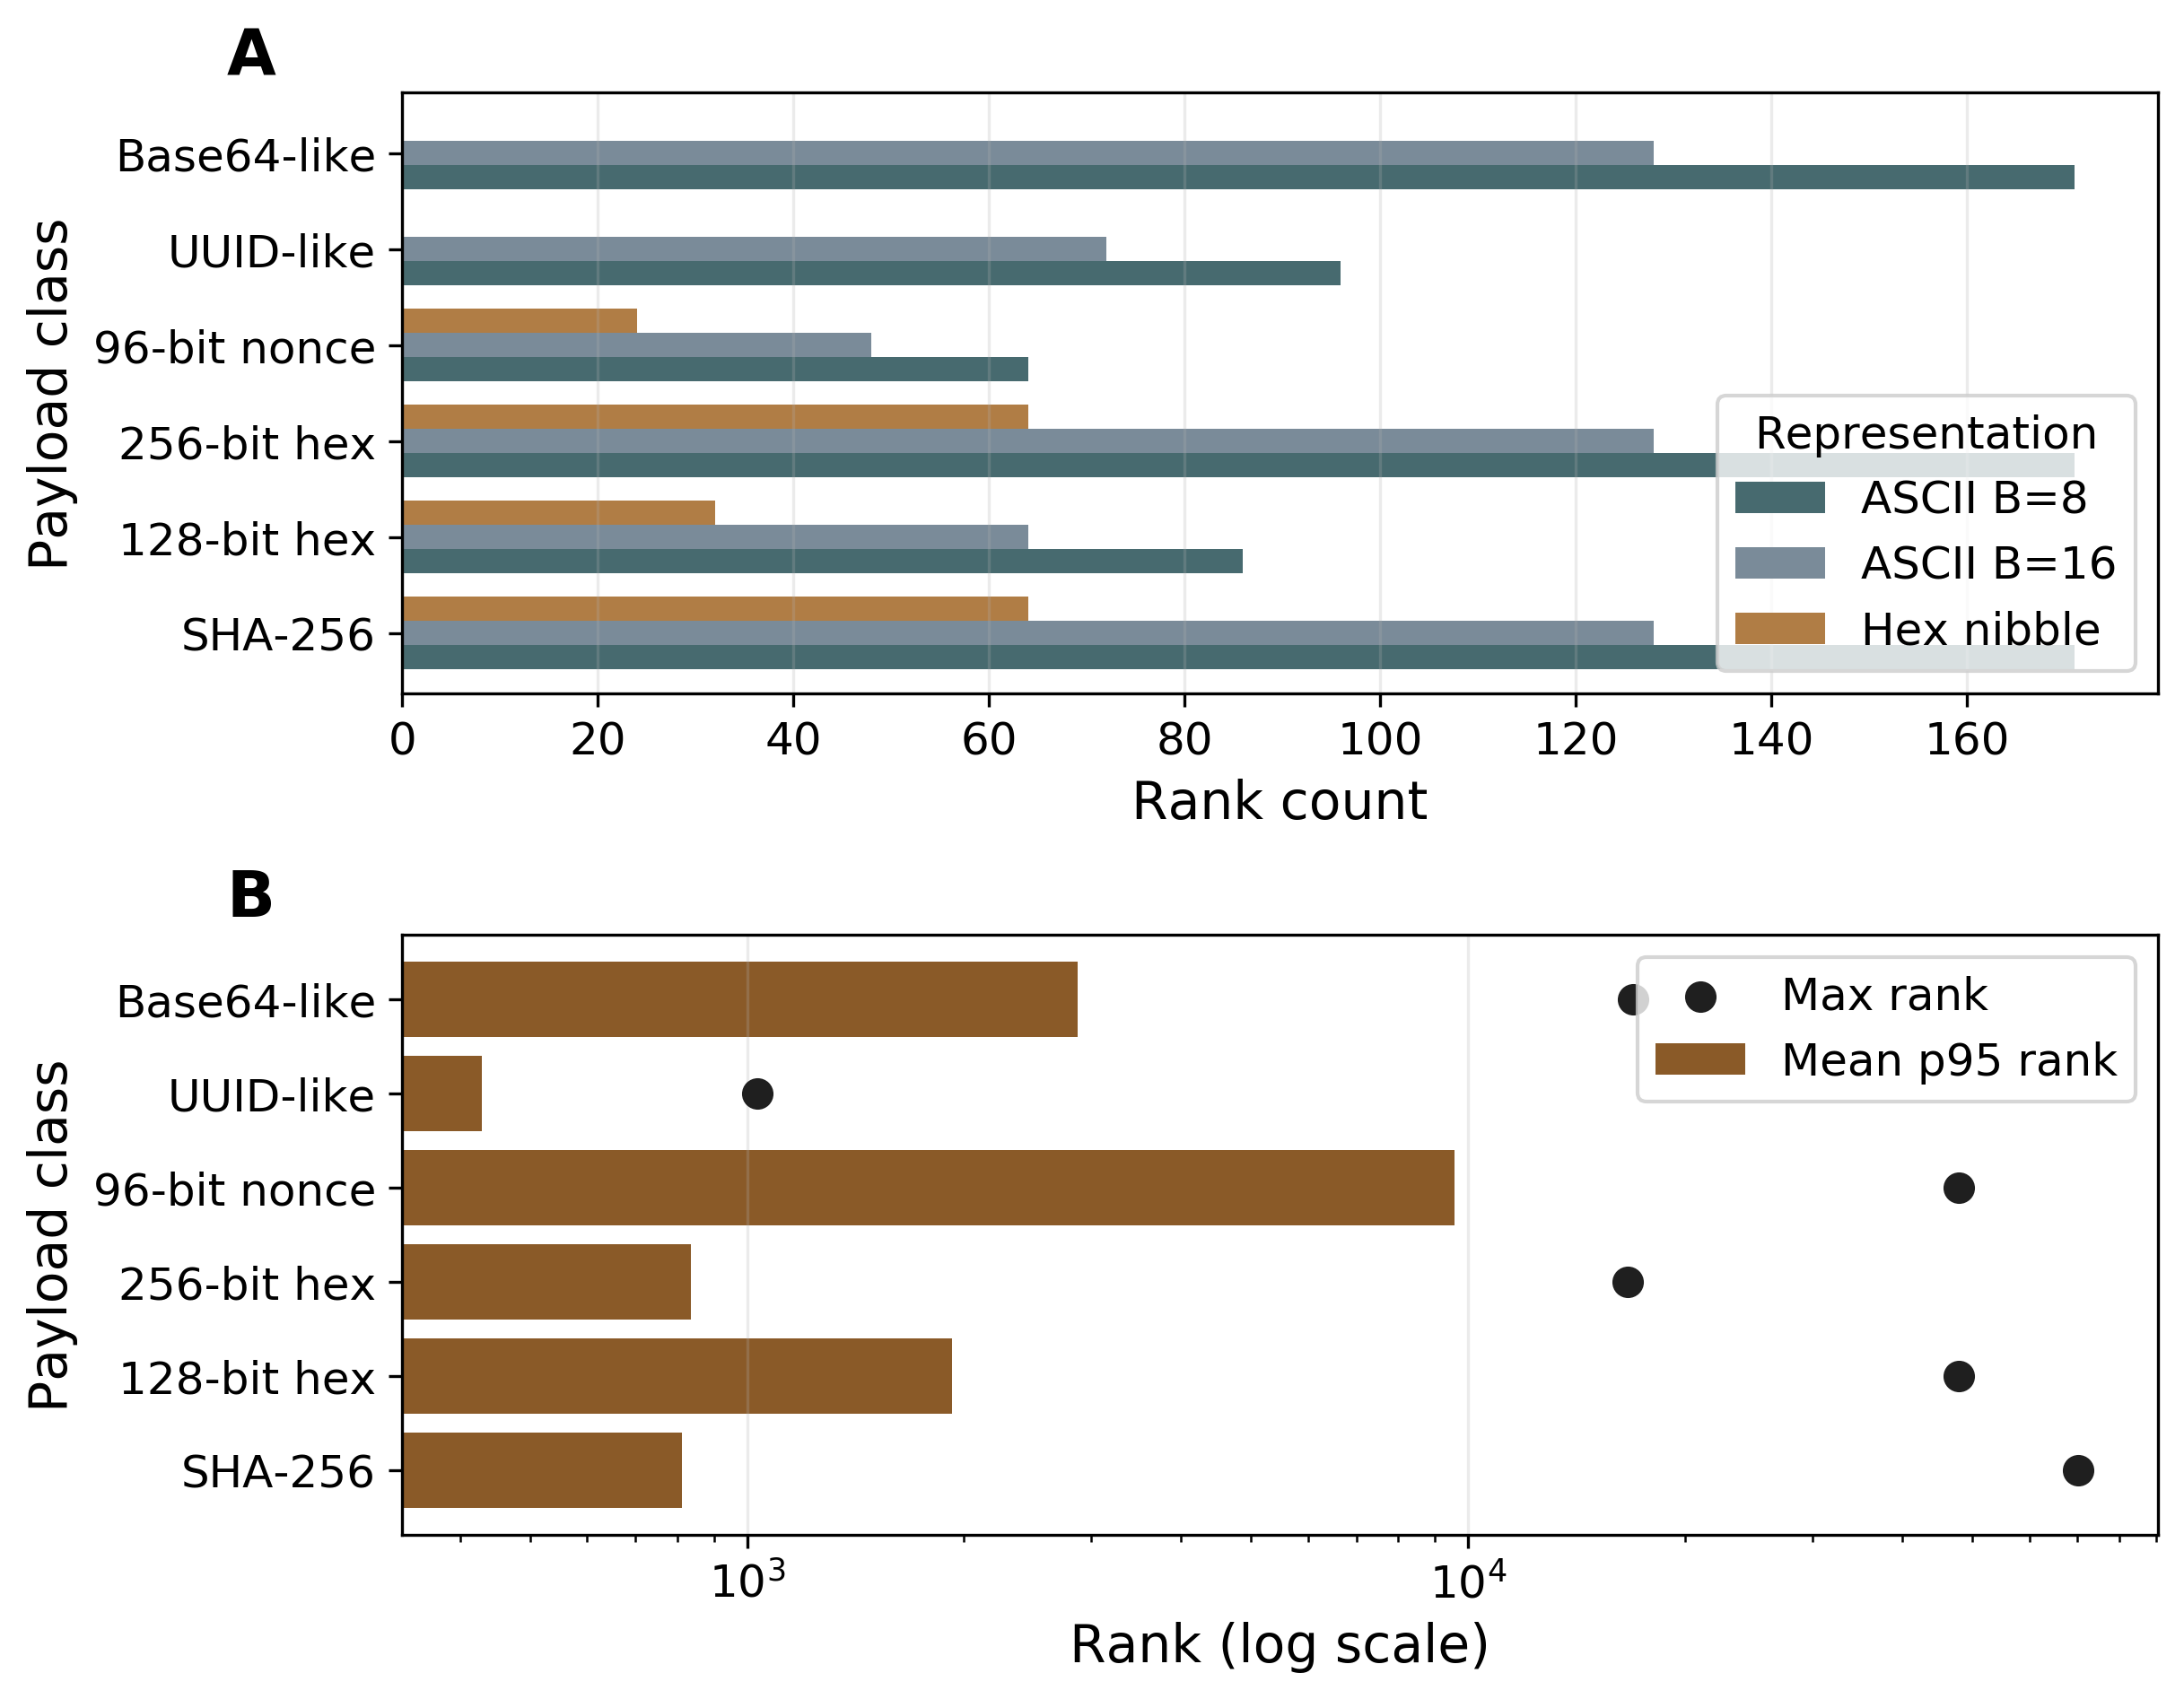
\includegraphics[width=0.95\linewidth]{figures/paper_main_payload_rank_pressure.png}
\caption{\label{fig:representation}Payload representation and direct rank-pressure diagnostics from the completed payload diagnostics. Panel A compares deterministic codec rank counts by payload class. Panel B shows direct subword rank pressure on a log scale. Bounded-rank encodings constrain possible requested ranks but increase rank count relative to direct subword tokenization. Direct subword tokenization can be compact but produced large observed ranks for several synthetic artifact classes.}
\end{figure}

Table~\ref{tab:payloads} and Figure~\ref{fig:representation} together show why RankCloak treats payload representation as a separate experimental object. The bounded-codec rows make rank pressure predictable by construction: ASCII-byte \(B=8\) maps displayed bytes into ranks \(1,\ldots,8\), ASCII-byte \(B=16\) maps displayed bytes into ranks \(1,\ldots,16\), and raw hex-nibble coding maps lowercase hex characters into ranks \(1,\ldots,16\). Both ASCII-byte codecs applied to all 12 payload rows and round-tripped exactly at the codec level, while raw hex-nibble coding applied to the 8 hex-like payload rows and did not apply to UUID-like or base64-like rows. The rank-count differences follow directly from the mappings in Eq.~\eqref{eq:hex-nibble-map} and Eq.~\eqref{eq:ascii-radix-map}: for SHA-256 and random 256-bit hex payloads, ASCII-byte \(B=16\) required 128 ranks, whereas raw hex-nibble coding required 64 ranks. For random 128-bit hex payloads, ASCII-byte \(B=16\) required 64 ranks, whereas raw hex-nibble coding required 32 ranks. The result is the first main finding: direct subword representation is compact but uncontrolled, while bounded-rank representation is longer but rank-limited.



\subsection*{Completed non-segmented trials recover exactly but show a capacity-quality tradeoff}

The completed non-segmented rows test the simplest RankCloak setting with one synthetic payload is encoded into one bounded rank sequence, one public cover text is generated from those ranks, and the receiver decodes by replaying the exact generated token sequence. In this setting, all completed non-segmented rows recovered exactly, 20 of 20 completed trials decoded back to the original displayed payload. This shows that the bounded-codec mechanism works under the exact-copy replay condition for the completed rows. In practical terms, the artifact string that would normally appear as visible hex, UUID-like text, or base64-like text was instead carried by the sequence of token choices in the generated cover.
Exact recovery, however, is not the same as equally natural cover text. Each payload rank tells the model which ranked token to choose at a particular point in the message. Small ranks usually select tokens the model already considered likely, while larger ranks force the model farther from its preferred continuation. The message can still decode correctly, but the public text may become less fluent, less typical under the model, or more likely to contain visible artifacts.
The completed subset contains 8 ASCII \(B=8\) rows, 6 ASCII \(B=16\) rows, and 6 hex-nibble rows. These variants represent different choices in the same capacity-quality tradeoff. ASCII \(B=8\) uses only ranks \(1,\ldots,8\), so it tends to choose from a more probable part of the model distribution, but it requires more generated tokens to carry the same payload. ASCII \(B=16\) and hex-nibble coding can be more compact, especially for hex payloads, but they allow larger requested ranks and can put more pressure on local token choices. The interpretation is that hiding the payload in fewer words can make each word choice harder.

Figure~\ref{fig:capacityquality} visualizes this tradeoff. Panel A compares completed non-segmented bounded-rank variants by generated length and mean token log probability. Longer covers indicate that more generated tokens were needed to carry the payload, while less negative log-probability values indicate that the generated tokens were more likely under the model. In the completed rows, ASCII \(B=8\) produced longer covers but had the strongest mean token log-probability proxy, while hex-nibble coding produced shorter covers for hex payloads but had lower mean token log probability. This pattern supports the RankCloak motivation as the codec choice controls the balance between cover length and how strongly the payload forces the model away from its preferred text.
Panel B adds segmented full public messages to the same length-quality plane. These points must be interpreted separately because segmented full-message values include non-payload natural tails. Tails can improve the full public message by adding easy, high-probability continuation tokens, but they do not carry payload ranks and are ignored by the decoder. Thus Panel B shows how public-message quality changes when tails are included where it does not show that the payload-bearing forced spans themselves are equally natural.

The recovery result also clarifies why failures can occur. RankCloak depends on replaying the same sequence of model contexts. Edits, paraphrases, whitespace changes, truncation, retokenization, model changes, prompt changes, or filter changes can alter the recovered ranks. Failures can also occur when extra text is inserted before the payload-bearing region and the receiver does not reproduce that boundary exactly. This is why the experimental lead-in variant is shown separately: it may make a message begin more naturally, but it adds a replay condition before decoding. The observed lead-in failure supports the methodological choice to measure replay boundaries, payload-bearing spans, and non-payload continuations separately.
Overall, the completed non-segmented rows support the main RankCloak methodology. Bounded codecs can make synthetic artifact payloads exactly recoverable under controlled replay, but recovery alone is not enough. RankCloak makes the tradeoff measurable where lower-rank codecs can improve model-typical token choices at the cost of longer covers, while more compact codecs reduce length but can increase pressure on the generated text.

\begin{figure}[ht]
\centering
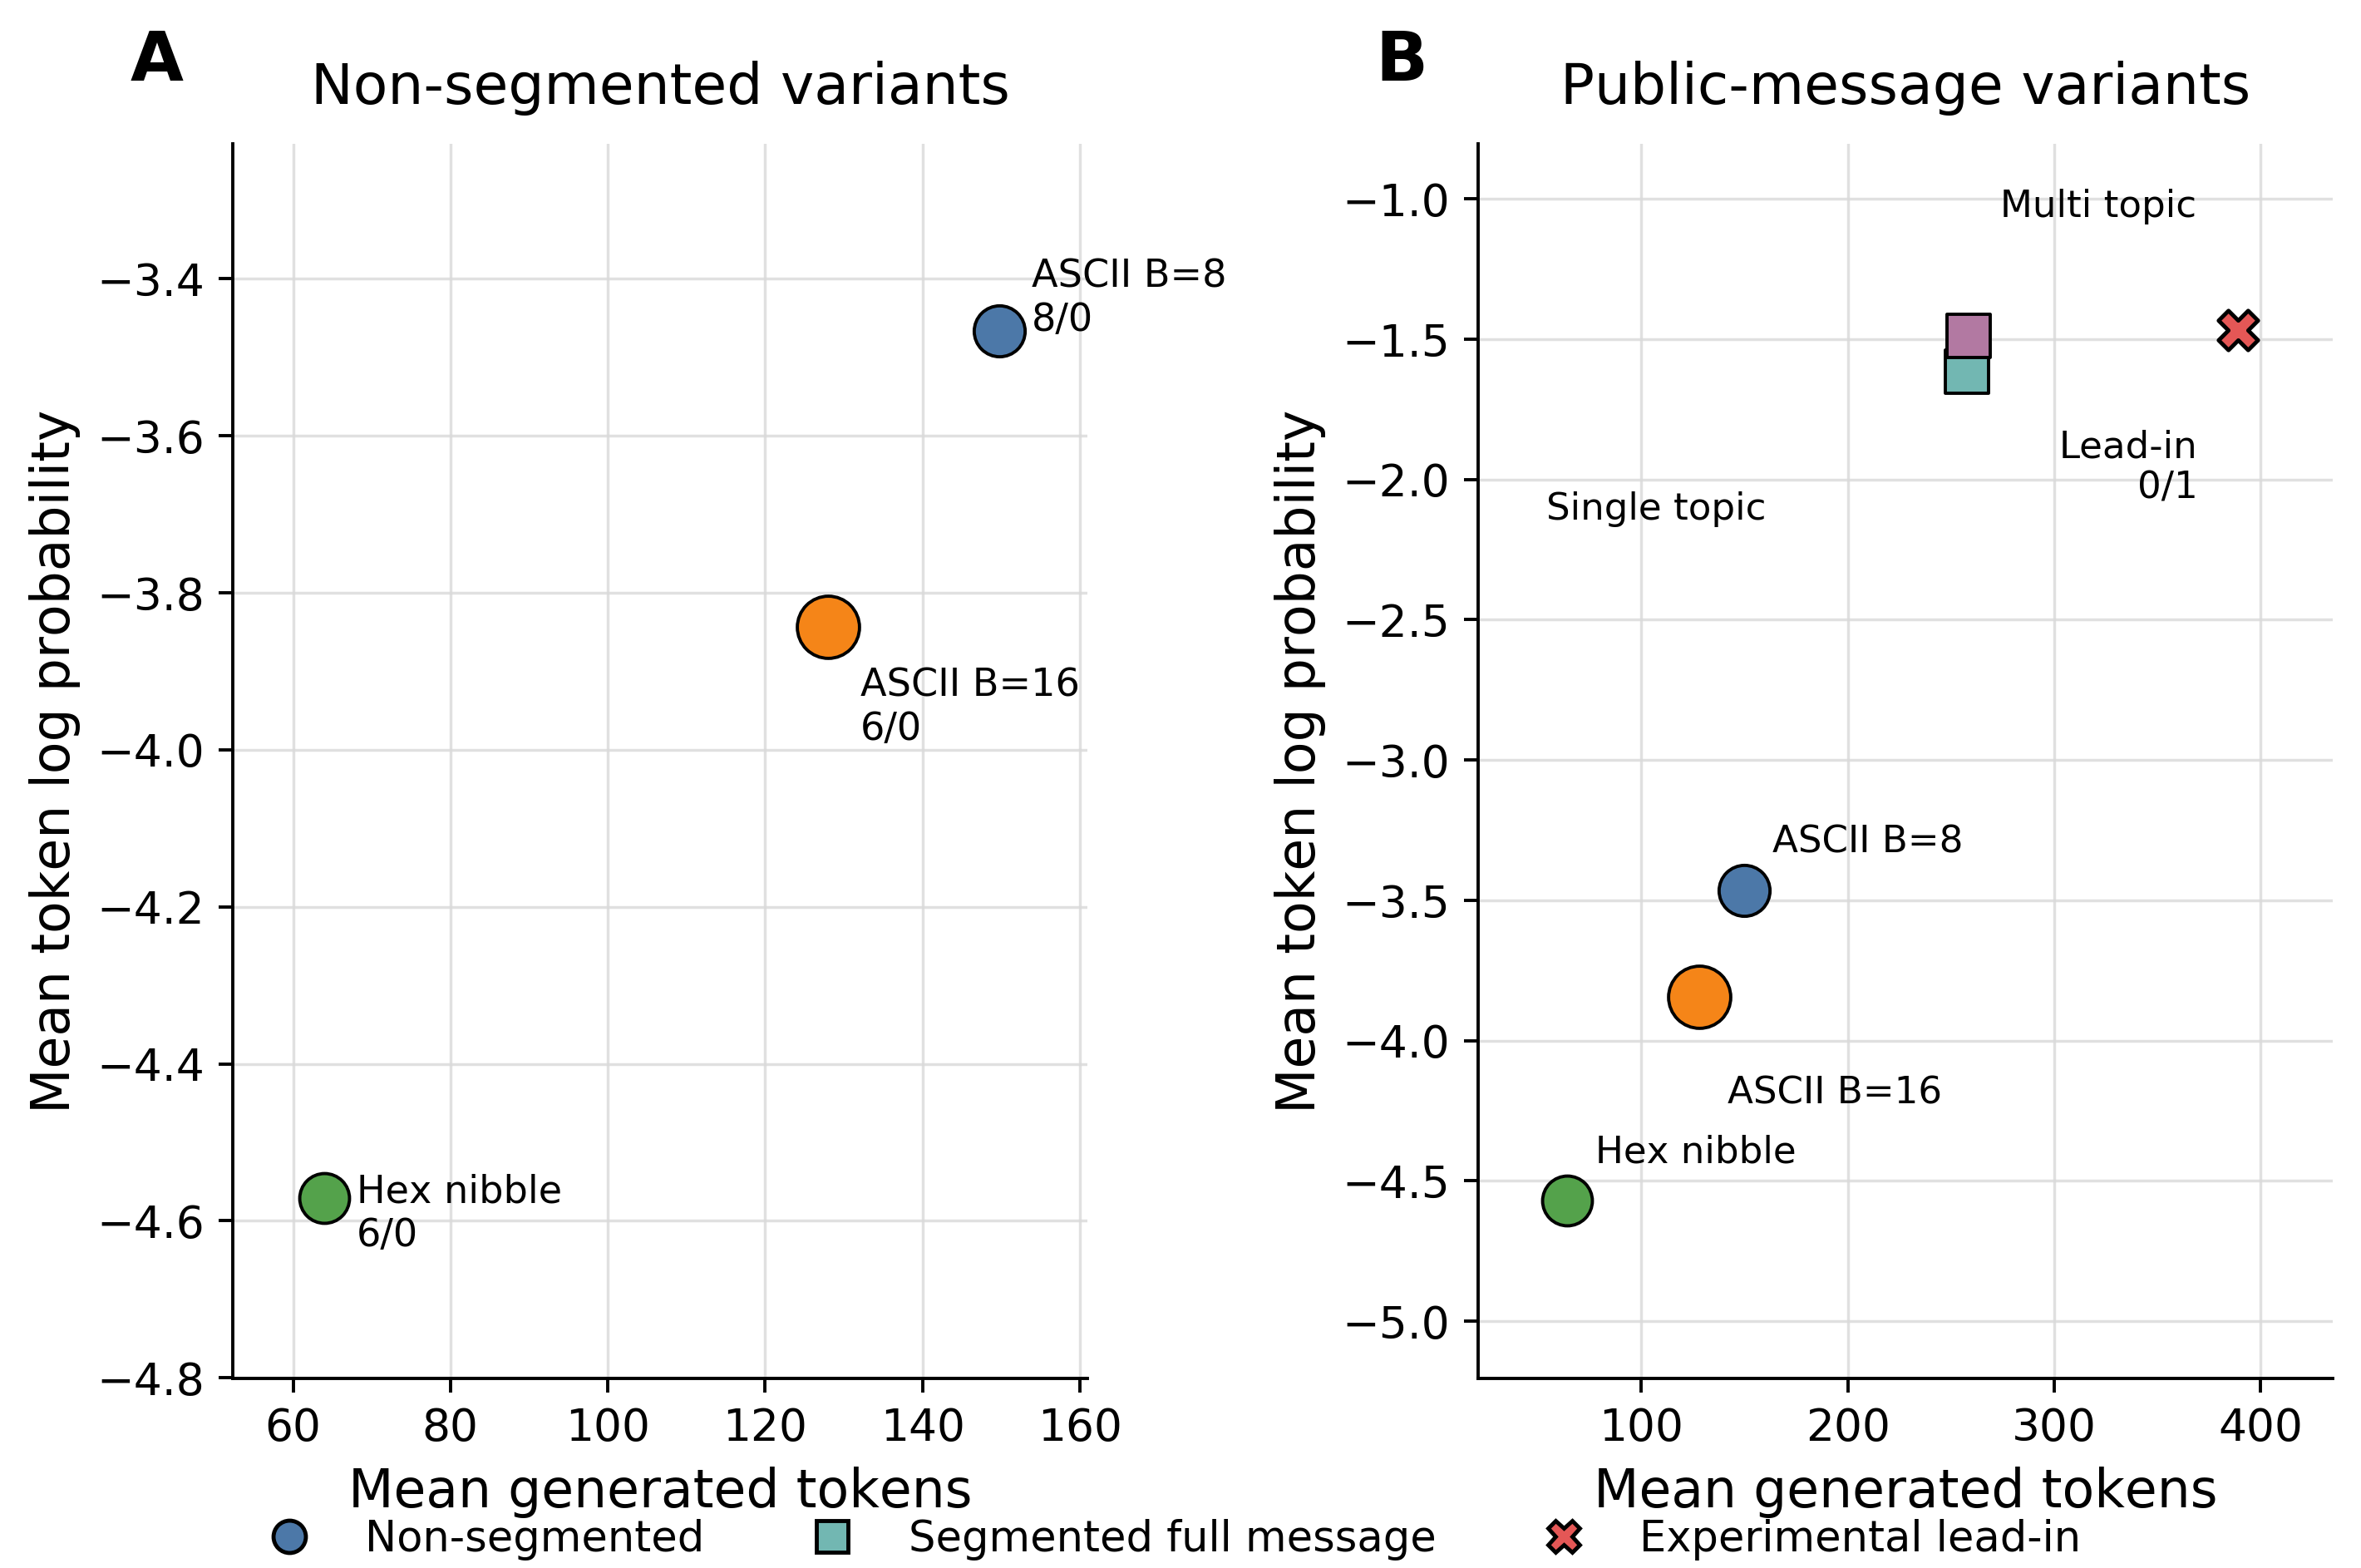
\includegraphics[width=0.95\linewidth]{figures/paper_capacity_quality_frontier.png}
\caption{\label{fig:capacityquality}Capacity-quality frontier for completed cover-generation trials. Panel A compares completed non-segmented bounded-rank variants by generated length and mean token log-probability proxy. Longer covers indicate that more generated tokens were needed to carry the payload, while less negative log-probability values indicate that the generated tokens were more likely under the model. Panel B places non-segmented rows and segmented full public-message rows on the same length-quality plane. Segmented full-message values include non-payload natural tails, so they should not be interpreted as payload-bearing forced-span quality. Point area scales with mean deterministic artifact flags. The experimental lead-in variant is shown separately because it has one observed exact-recovery failure.}
\end{figure}




\subsection*{Segmented variants separate recovery correctness from public-message quality}

The segmented rows recovered exactly in 6 of the 7 completed trials.
In this setting, a payload is not carried by one long generated cover. Instead, it is split across several short payload-bearing spans, and each span is placed inside a separate public message.
These rows use Algorithm~\ref{alg:segmented}; recovery uses only the forced spans defined in Eq.~\eqref{eq:segmented-forced-span}. The non-lead-in segmented variants each recovered in all completed rows, 3 of 3 for segmented single-topic and 3 of 3 for segment multi-topic. The only observed failure was the single completed segmented lead-in row, which used an eight-token greedy lead-in before the forced span. This failure is informative because the lead-in changes the context that must be reproduced before decoding. If the receiver does not reconstruct that boundary exactly, the same forced tokens can map to different recovered ranks. This is why the lead-in variant is treated as experimental here.

Table~\ref{tab:protocolquality} summarizes the completed result rows by protocol variant and, importantly, shows which part of the generated text each metric describes. For non-segmented rows, token count, log probability, and artifact count describe the full generated cover. Thus the segmented rows should not be compared with the non-segmented rows as if all values measured the same kind of text. For segmented rows, these columns describe full public messages, which include non-payload natural tails. Supplementary Fig. S3 provides the corresponding artifact-flag diagnostic by protocol variant. It shows where the deterministic string-feature checks found markup-like or formatting artifacts in the completed rows. These flags are useful for auditing obvious generated-text problems, but they are not a human naturalness score and do not replace a dedicated steganalysis or readability study. Recovery is reported as pass/fail counts, so \(3/0\) means three completed rows recovered exactly and zero failed.

\begin{table}[ht]
\centering
\footnotesize
\setlength{\tabcolsep}{3pt}
\begin{tabular}{L{0.14\linewidth} r L{0.08\linewidth} L{0.14\linewidth} r r r L{0.18\linewidth}}
\toprule
Variant & Completed & Recovery & Metric scope & Mean tokens & Mean log prob. & Artifact flags & Status \\
\midrule
ASCII \(B=8\) & 8 & 8/0 & Full cover & 149.8 & -3.466 & 0.75 & Exact in completed rows \\
ASCII \(B=16\) & 6 & 6/0 & Full cover & 128.0 & -3.843 & 1.67 & Exact in completed rows \\
Hex nibble & 6 & 6/0 & Full cover & 64.0 & -4.571 & 0.67 & Hex-like only \\
Seg. single-topic & 3 & 3/0 & Full message with tail & 257.7 & -1.616 & 0.21 & Full message includes tails \\
Seg. multi-topic & 3 & 3/0 & Full message with tail & 258.3 & -1.486 & 0.21 & Full message includes tails \\
Seg. lead-in & 1 & 0/1 & Full message with tail & 389.0 & -1.467 & 0.00 & Experimental; one failure \\
\bottomrule
\end{tabular}
\caption{\label{tab:protocolquality}Completed recovery and cover-quality summary by protocol variant. Segmented log-probability values are full-message values and include non-payload natural tails. The table reports partial-pilot evidence only.}
\end{table}

Segmented rows separate payload-bearing forced-span metrics from full public-message metrics. The forced/full split follows from Eq.~\eqref{eq:segmented-message} and Algorithm~\ref{alg:tail}: tails are part of the public message but not part of the decoded rank sequence. The forced-span/full-message comparison asks a simple question: are we scoring the tokens that actually carry the payload, or the whole message seen by a reader? In segmented rows, only the forced span is decoded into ranks. The tail is visible public text, but it is a greedy non-payload continuation and is ignored by the decoder. Mean token log probability is used here as a model-based quality proxy; less negative values indicate text that the model considered more likely. Across the 7 completed segmented rows, the effect-size table reports a mean forced-span log probability of \(-5.274\) and a mean full-message log probability of \(-1.539\), a difference of 3.735 in favor of the full-message metric. This gap is expected because the full message includes easy greedy tail tokens. The result therefore supports the reporting convention: tails can improve the public-message proxy, but they do not show that the payload-bearing span itself became natural.

Figure\ref{fig:forcedfull} shows the aggregate forced-span versus full-message comparison, and Supplementary Table S3 gives the per-variant values. The supplementary table is important because it shows that full-message log-probability proxies are much higher after tails are included, but this does not mean the payload-bearing forced span itself improved. The segment lead-in row also shows why recovery correctness and public-message quality must be reported separately, because that experimental row failed exact recovery despite having the highest full-message proxy in the table.

\begin{figure}[htbp]
\centering
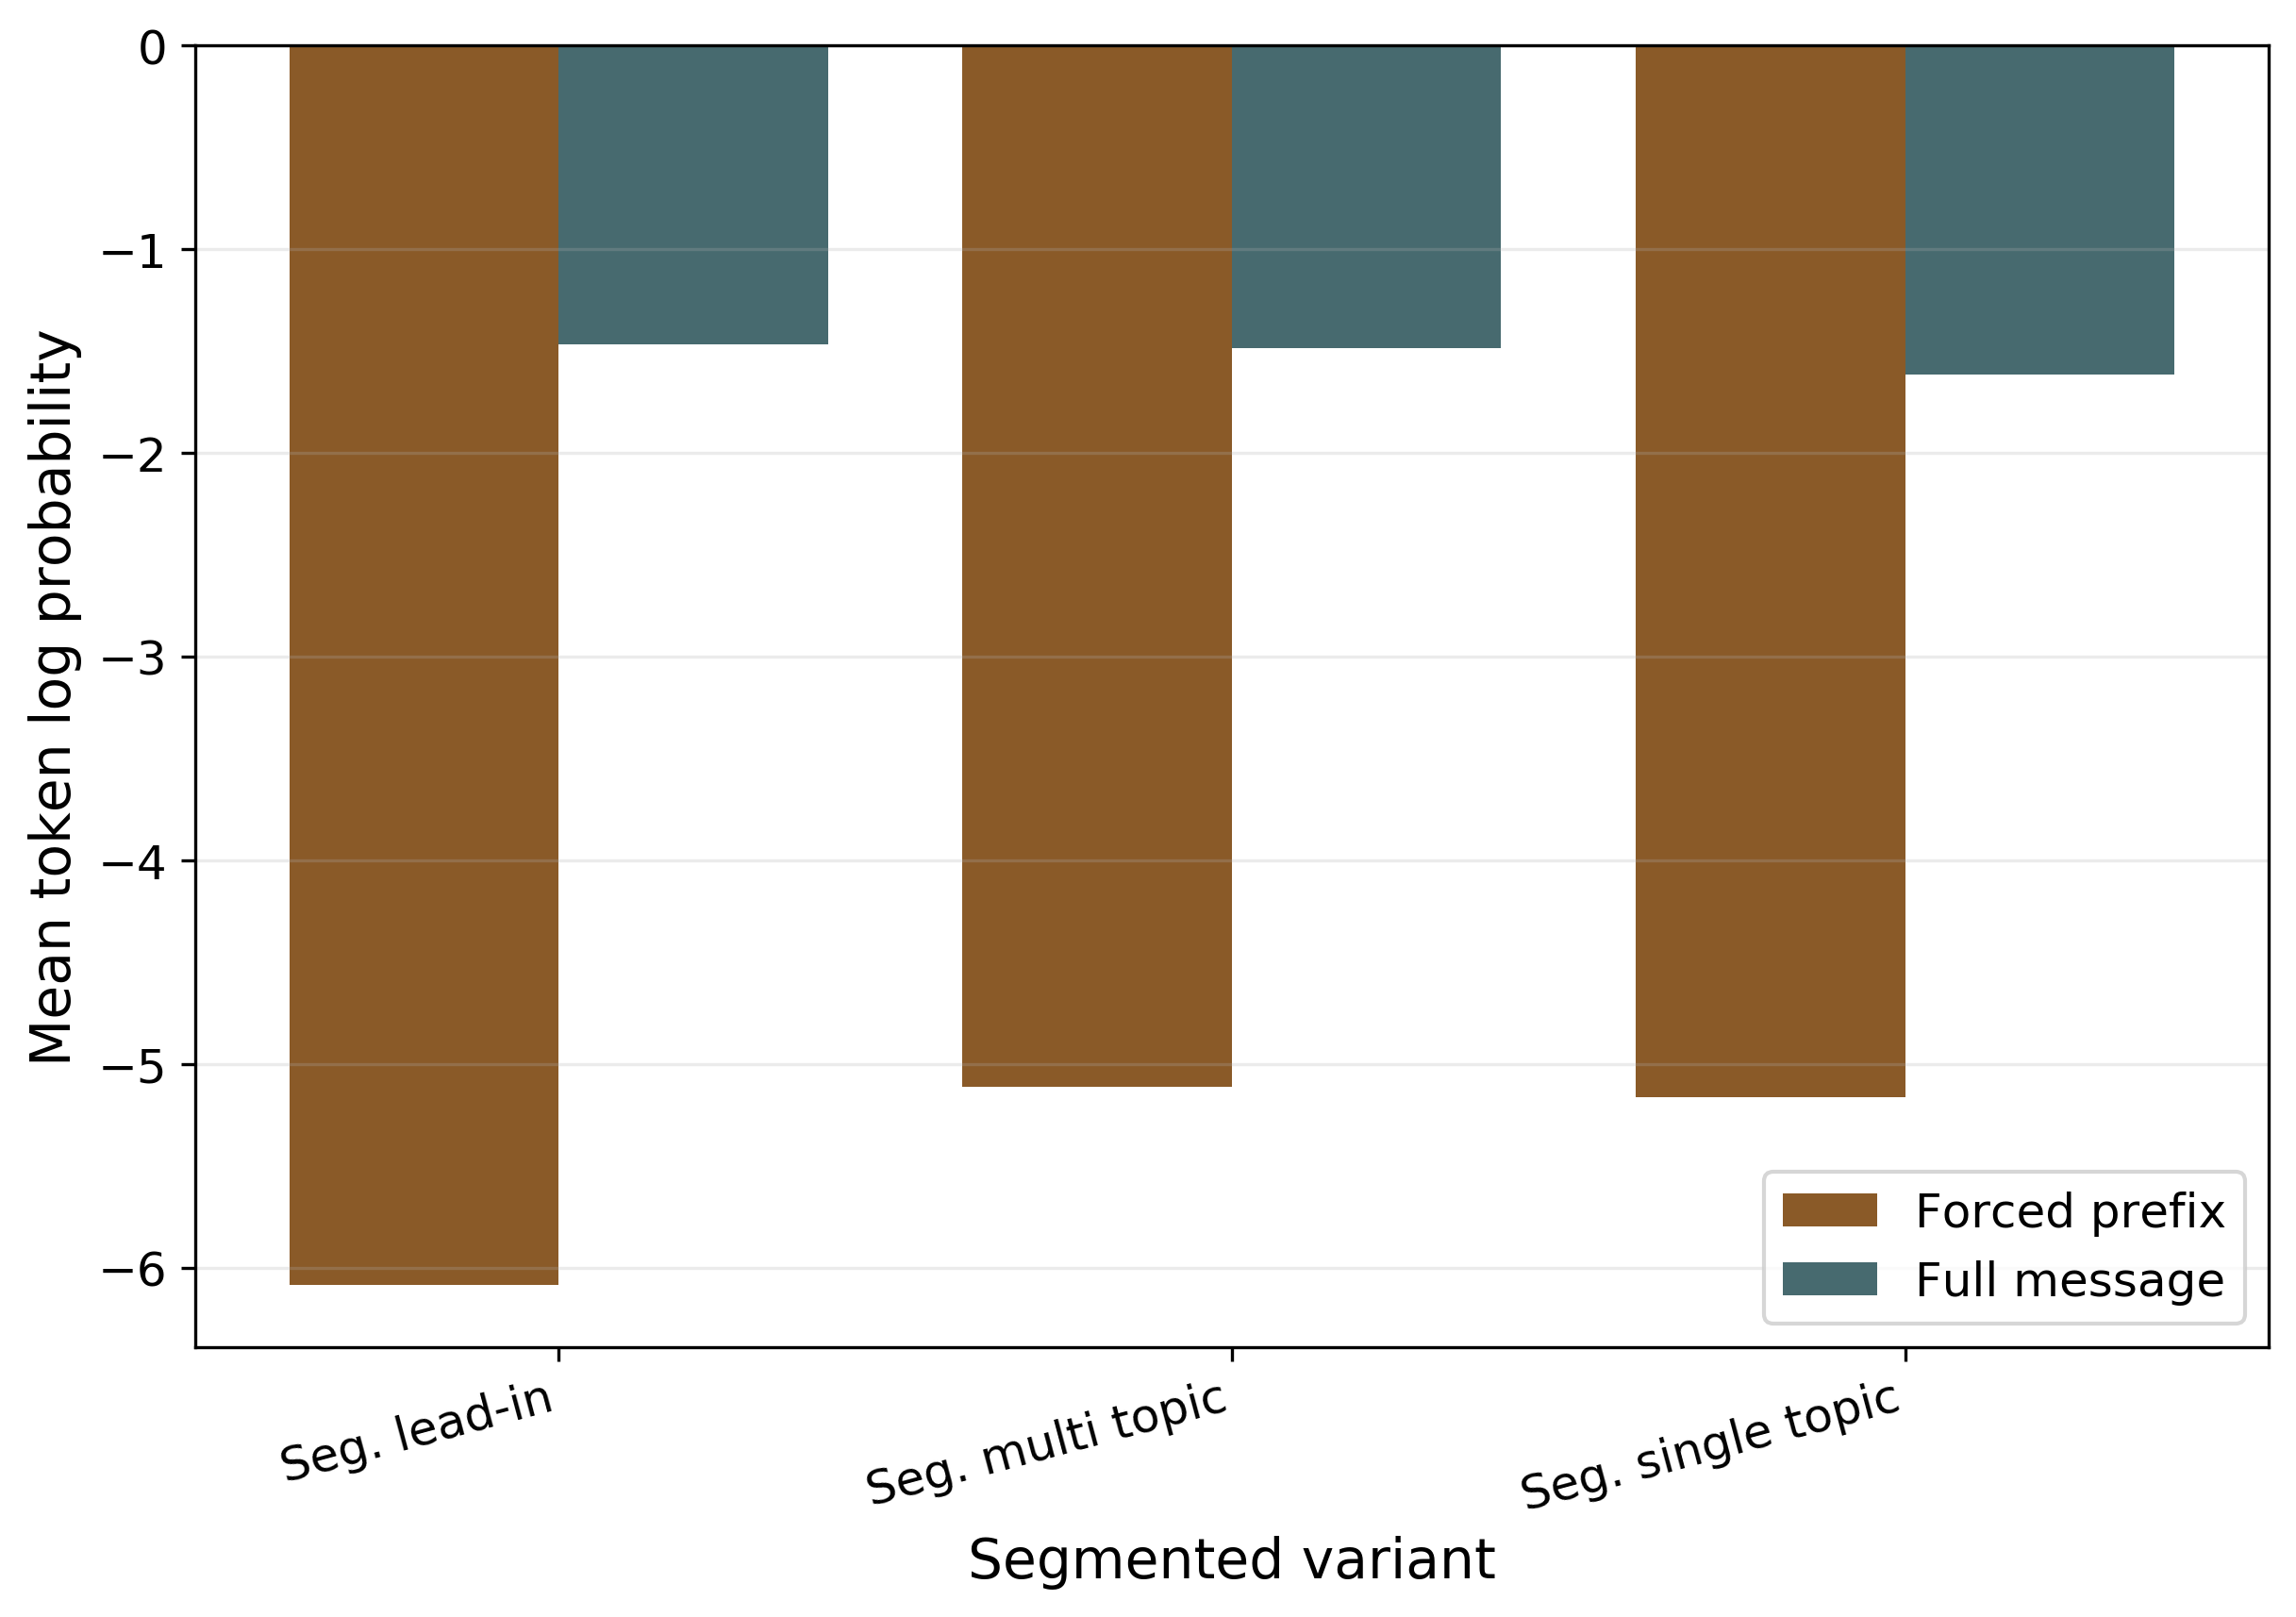
\includegraphics[width=0.95\linewidth]{figures/paper_forced_prefix_vs_full_message.png}
\caption{\label{fig:forcedfull}Forced-span versus full-message metrics for completed segmented trials. Full-message metrics include greedy natural tails and can look substantially better than payload-bearing forced-span metrics. The comparison is used to show when apparent public-message quality is driven by non-payload continuation text rather than by the tokens that carry the payload.}
\end{figure}

Figure~\ref{fig:tailtopic} asks whether the same tail effect appears across prompt topics. For each completed segment, tail gain is computed as the full-message mean token log probability minus the forced-span mean token log probability. This is a before-and-after public-message difference, not a likelihood assigned only to the tail. Positive tail gain means that adding the non-payload continuation improved the full-message proxy, while the decoded payload-bearing span remained the same.The topic-level diagnostic includes 48 completed segmented messages across five prompt labels. In these partial rows, the mean tail-gain proxy ranged from 3.688 for plant-care notes to 4.113 for recipe-blog prompts, with uneven topic counts from 3 to 27 segments. Some topic bins include segments from the experimental lead-in failure, so the result is a prompt-topic diagnostic rather than a final prompt ranking. Figure\ref{fig:tailtopic} shows the topic-level pattern, and Supplementary Table S5 gives the numeric topic summaries. The supplementary table reports segment counts, forced-span mean log probability, full-message mean log probability, tail gain, average tail length, artifact flags, and segment-level recovery counts for each prompt topic. These values should be read as topic diagnostics rather than as a final prompt ranking because the topic bins are uneven and some include segments from the experimental lead-in condition. Because the topic bins are uneven and some include segments from the experimental lead-in condition, these values should be read as topic diagnostics rather than as a final prompt ranking.

\begin{figure}[htbp]
\centering
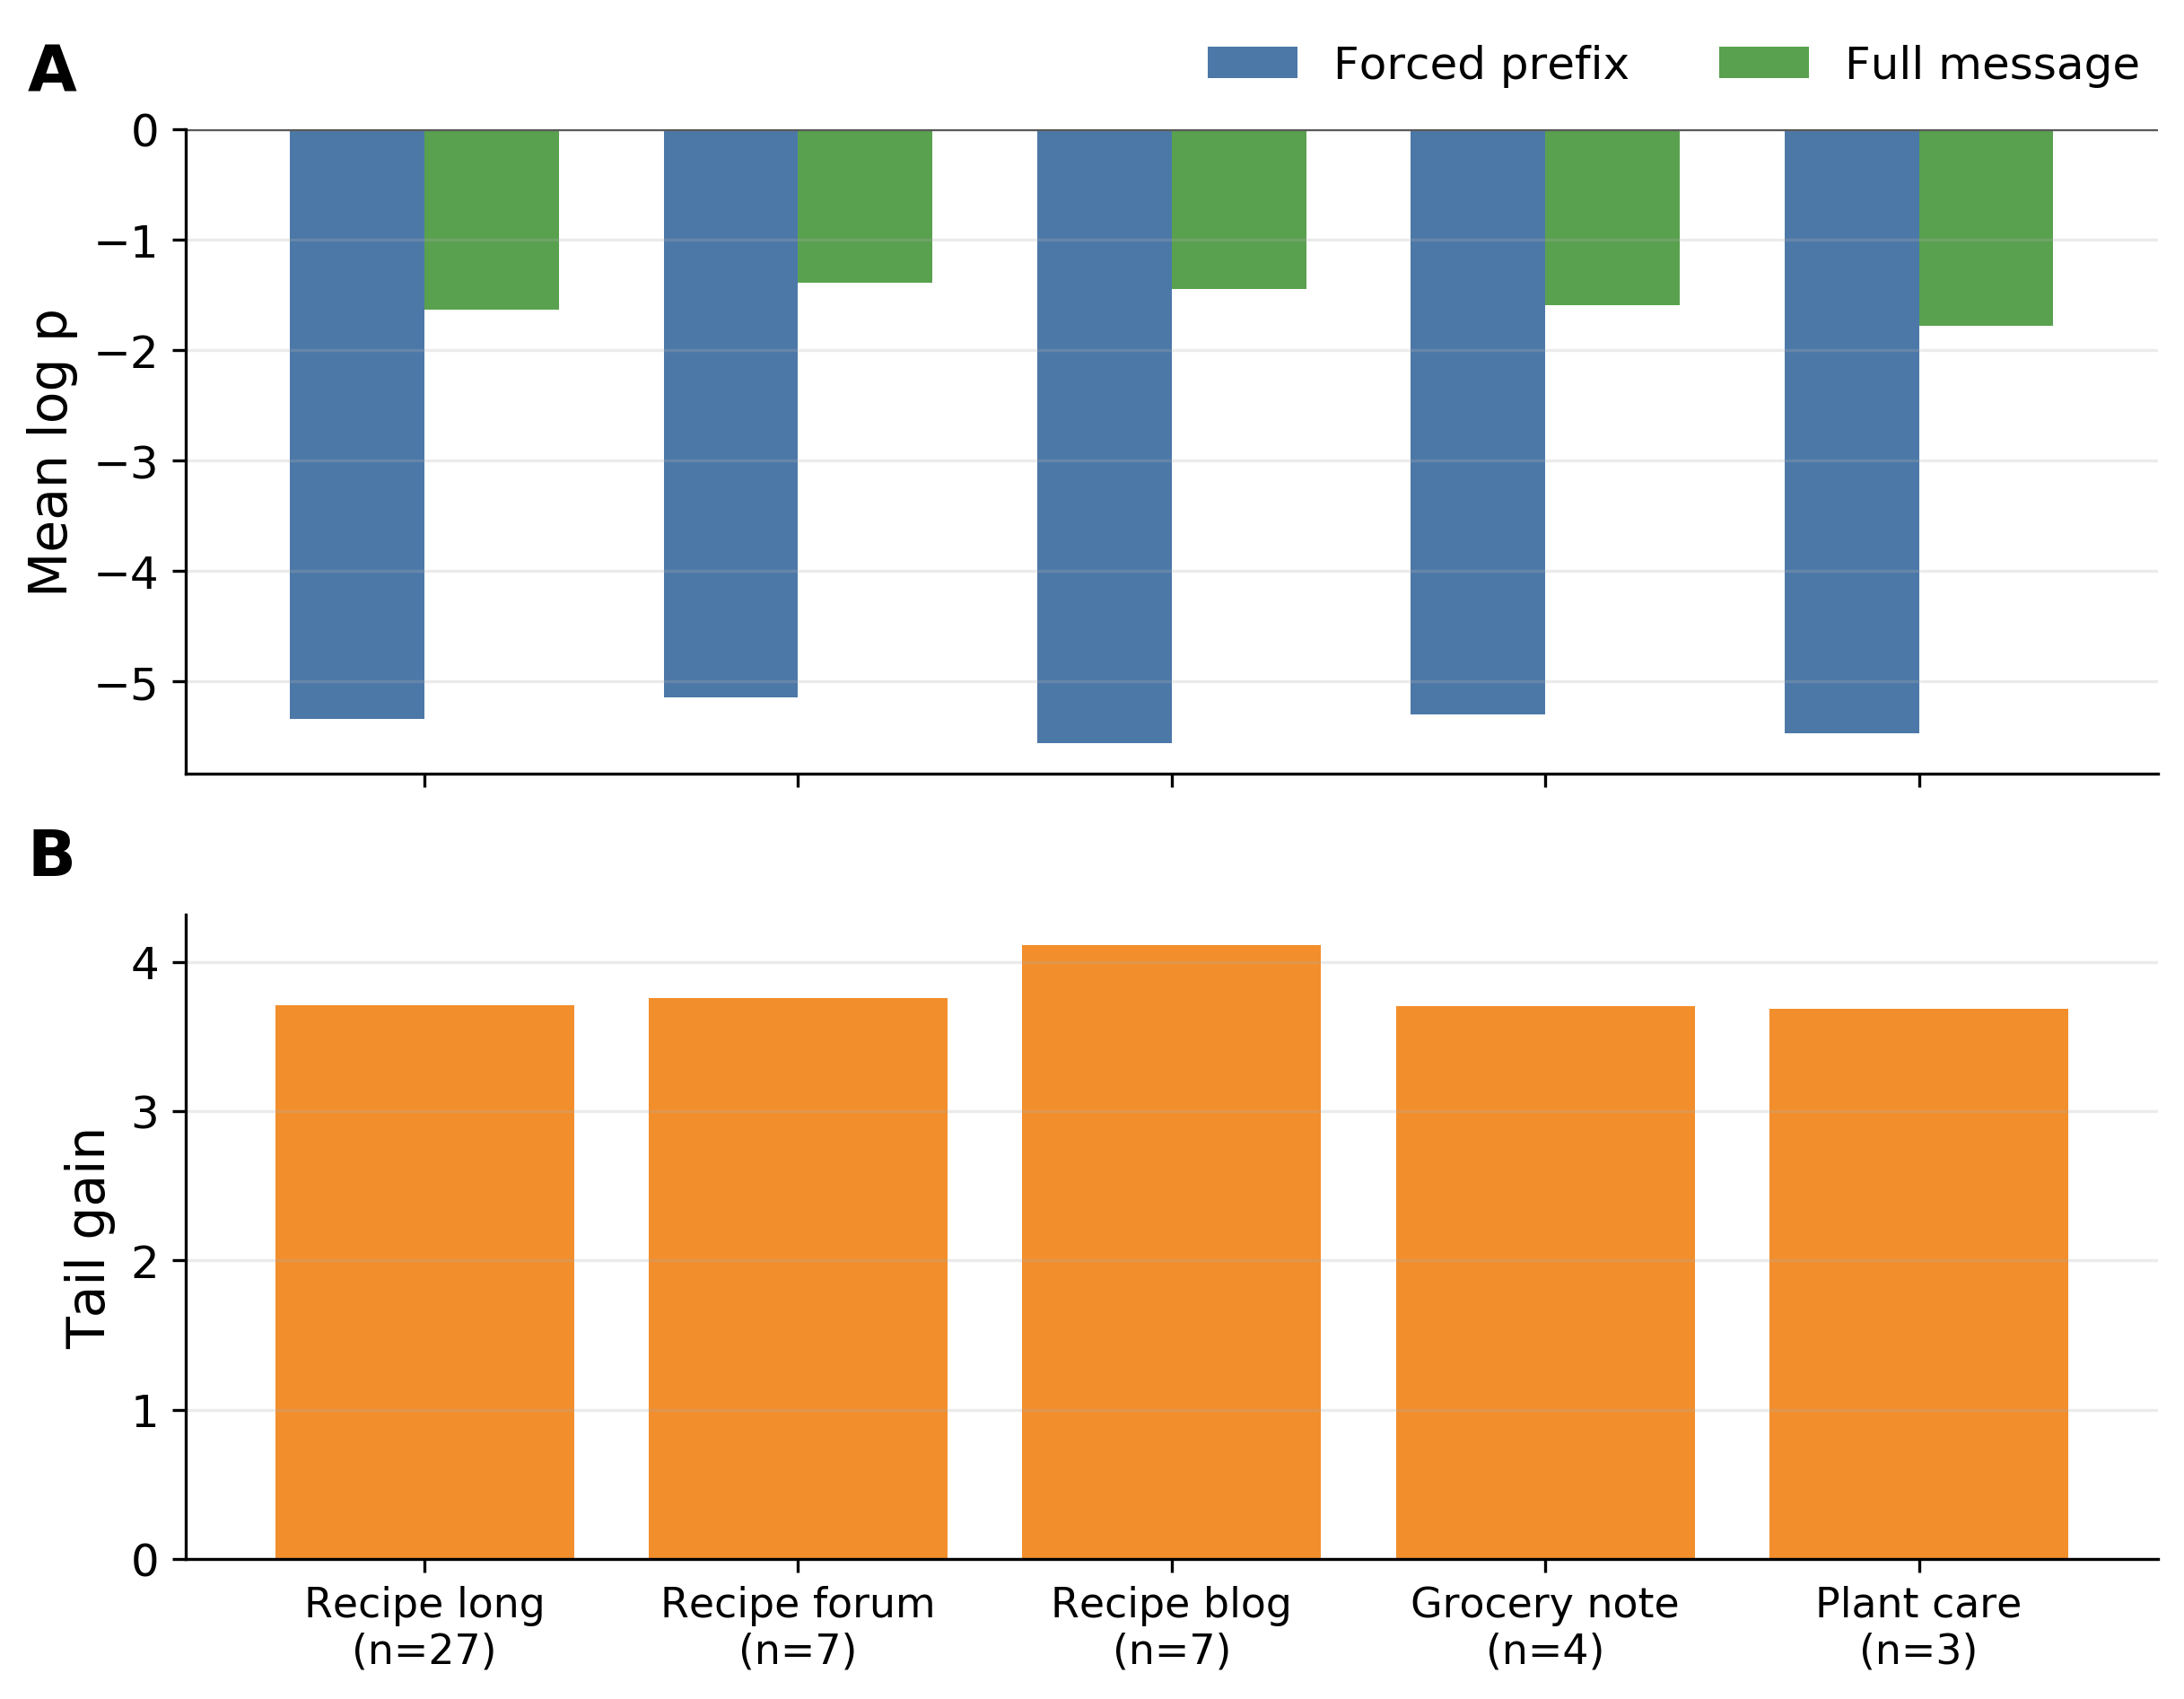
\includegraphics[width=0.95\linewidth]{figures/paper_tail_topic_quality.png}
\caption{\label{fig:tailtopic}Tail-topic quality diagnostic for completed segmented messages. In the vertical axis label, mean log \(p\) denotes mean token log probability. Tail gain is the full-message mean token log probability minus the forced-prefix mean token log probability (it is not a tail-only likelihood). Tail tokens are greedy non-payload continuations, carry no payload ranks, and are ignored by the decoder.}
\end{figure}


These aggregate metrics above can obscure the simple mechanics of the method, so Table~\ref{tab:examples} gives a short decoding trace for one synthetic hex-like payload fragment. The table illustrates the same hex-nibble mapping in Eq.~\eqref{eq:hex-nibble-map} and the forced-span/tail distinction in Algorithm~\ref{alg:segmented}. It shows how a truncated payload fragment is converted into hex-nibble ranks, how those ranks select the payload-bearing cover span, and how the receiver recovers the original fragment by replaying the exact forced tokens. A complete segmented example showing a full synthetic hex payload, its rank chunks, and all public cover messages is provided in the Supplementary Information.

\begin{table}[ht]
\centering
\scriptsize
\setlength{\tabcolsep}{3pt}
\begin{tabular}{L{0.19\linewidth} L{0.32\linewidth} L{0.39\linewidth}}
\toprule
Step & Example fragment & Decoder meaning \\
\midrule
Synthetic payload excerpt & \texttt{744ffb44...} & Truncated excerpt from a deterministic synthetic SHA-256-like artifact; not a real secret. \\
Hex-nibble ranks & \texttt{7 4 4 f f b 4 4} \(\rightarrow\) \texttt{8,5,5,16,16,12,5,5} & Each lowercase hex digit maps to one bounded rank in \(1,\ldots,16\), with \texttt{0}\(\rightarrow 1\) and \texttt{f}\(\rightarrow 16\). \\
Cover prompt and segment & recipe long, segment 1, 8 forced ranks & The prompt defines the cover distribution; the segment size defines how many payload-bearing tokens are decoded. \\
Forced cover span & ``Here's your opportunity--finally the arom'' & These exact received forced-span tokens carry the ranks and are replayed by the decoder. \\
Natural tail & ``atics are softening, and the pot is filling\ldots{}'' & Greedy non-payload continuation; public text after the forced span is ignored by the decoder. \\
Recovery & \texttt{8,5,5,16,16,12,5,5} \(\rightarrow\) \texttt{744ffb44...} & The receiver replays the exact forced span, recovers the same ranks, and decodes the truncated payload fragment. \\
\bottomrule
\end{tabular}
\caption{\label{tab:examples}Worked payload-to-cover example for a segmented hex-nibble row. The payload excerpt is synthetic and truncated. Hex-nibble coding maps each lowercase hex character to a rank in \(1,\ldots,16\). The forced cover span carries the payload ranks; the natural tail is public non-payload text and is ignored by the decoder. The table is illustrative and does not claim human naturalness, undetectability, encryption, or cryptographic security.}
\end{table}

Supplementary Example S1 gives the complete segmented instance corresponding to this mechanism. It lists the full synthetic SHA-256-like payload, all eight hex-nibble rank chunks, the forced spans, the non-payload tails, and the recovered payload. The example reinforces the central segmented-result interpretation: recovery uses only the forced spans, while the tails affect the public message but do not carry payload ranks.
Additional shortened examples in the Supplementary Examples section compare a validated single-topic segmented row with the experimental failed lead-in row. These examples are useful for seeing the practical difference between the validated forced-span/tail structure and the extra boundary-replay condition introduced by the lead-in variant.




\subsection*{Diagnostics and staged-evaluation scope}

The main Results above are based on the completed staged RankCloak rows, payload-representation diagnostics, non-segmented cover-generation trials, and segmented cover-generation trials. The software repository also contains exploratory pilots and auxiliary diagnostic outputs that informed the final methodology. 
Supplementary Table S4 gives the cross-pilot synthesis. Across the earlier pilots, a consistent pattern appears: exact recovery can be reliable under exact-copy replay, but public-message quality remains sensitive to rank pressure, prompt format, and protocol structure. Supplementary Fig. S4 visualizes the same development logic. Larger fixed-rank alphabets can reduce rank count while lowering the mean token log-probability proxy, and prompt-format changes can improve topic anchoring without eliminating forced-rank damage. These observations support the final RankCloak design: represent payloads explicitly, bound rank pressure where possible, restart context through segmentation, use tails to study public-message continuity, and report payload-bearing spans separately from full messages.

The feature-only detector outputs provide a diagnostic view of the recorded cover texts. The detector dataset contains 272 rows, and the detector output contains 57 result rows. These rows use numeric and Boolean cover features rather than raw text. Supplementary Fig. S1 reports AUC summaries for several views, including full public messages, non-segmented rows, segmented full messages, and payload-bearing forced spans. The purpose is to check whether simple features such as mean token log probability, artifact flags, and cover-quality summaries separate completed RankCloak rows from greedy prompt-matched baselines.
These detector results are measurement diagnostics, not security claims. A high AUC in the current feature views means that the recorded RankCloak outputs are distinguishable from the chosen greedy baselines under those features. It does not establish general detectability, undetectability, adversarial robustness, or performance against raw-text steganalysis. The value of the detector outputs is that they connect construction-side choices to detection-relevant features and provide a reproducible starting point for future steganalysis.




%%%%%%%%%%%%%%%%%%%%%%%%%%%%%%%
%%%%%%%%%%%%%%%%%%%%%%%%%%%%%%%
\section*{Discussion}

RankCloak shows that synthetic cryptographic artifacts, such as hash-like, UUID-like, and ciphertext-like strings, can be represented as sequences of LLM token ranks and recovered from generated English text when the exact token sequence and model configuration are preserved. In the evaluated subset, non-segmented bounded-codec rows recovered exactly in 20 of 20 trials, and segmented rows recovered exactly in the majority of trials. The result is a methodology for measuring how these artifacts can be carried by generated text, not a claim of secure deployment.
A central finding is that the payload representation matters. Direct subword tokenization can be short, but it can require the cover generator to choose tokens that are very unlikely under the public prompt. In the completed diagnostics, one SHA-256-style row reached a maximum direct rank of 70,108. This shows why hash-like and ciphertext-like payloads are difficult: they may look compact as strings, but they can push generation toward unnatural token choices.
The bounded codecs reduce this problem by converting the displayed artifact into a controlled rank sequence. ASCII-byte coding can represent arbitrary displayed byte strings, while hex-nibble coding is more efficient for lowercase hex payloads. For a 64-character hex artifact, hex-nibble coding uses 64 ranks rather than 128 ranks under ASCII-byte \(B=16\), while keeping every requested rank in \(1,\ldots,16\). The cost is that bounded representations can require more generated cover tokens. RankCloak makes this tradeoff visible by reporting recovery, cover length, and model-based quality measures separately.

Segmentation addresses a related problem. Instead of forcing one long cover text to carry a whole payload, segmented RankCloak splits a hex payload across several shorter public messages. Each message contains a payload-bearing forced span followed by a non-payload tail. This distinction is important because tails can make the full public message look better while carrying no payload ranks and being ignored by the decoder. Full-message quality should therefore not be treated as the quality of the hidden payload-bearing text itself.
The single lead-in failure is useful because it shows where the protocol is fragile. Adding natural-looking text before the forced span may make a message begin more smoothly, but it also creates another context that must be reproduced exactly before decoding. If that boundary is not replayed correctly, the recovered ranks can change. Future variants that add text before the payload-bearing span should therefore treat boundary alignment as a core part of the protocol.

The detector results also support the measurement view. They show that generated covers can leave measurable traces, including low-probability token choices, formatting artifacts, and differences between forced-span and full-message scores. This has defensive value: a detector looking for hidden cryptographic artifacts cannot rely only on visible patterns such as hex, base64, UUIDs, or credential-shaped strings. However, the current feature-only detector is a diagnostic baseline, not a complete steganalysis study or proof of detectability or undetectability.
Overall, RankCloak provides a controlled way to study how high-entropy synthetic artifacts can be transformed into plain-English LLM output through rank choices. The supported claim remains exact-copy and configuration-dependent that recovery requires the same model, tokenizer, quantization, prompts, rank ordering, codec, filter, segmentation policy, and generated token sequence. Within that scope, RankCloak makes the main tradeoffs visible, compact representations can damage cover quality, bounded ranks improve control but change length, and full public-message fluency can differ from the quality of the tokens that actually carry the payload. Future work entails investigating different tail strategies based on the codecs and how dynamic stopping criteria can be improved.




\section*{Data and code availability}

The source code and manuscript draft are in the repository \url{www.github.com/mantzaris/llm-rankcloak}. All data is synthetically generated.


\section*{Responsible use and limitations}

This manuscript uses only deterministic synthetic payloads and does not include real secrets, credentials, private keys, accounts, API tokens, operational commands, or service interactions. The evaluated setting is exact-copy recovery with a shared model/tokenizer/quantization/prompt configuration. The work does not claim encryption, key exchange, authentication, signing, credential protection, cryptographic security, undetectability, edit robustness, paraphrase robustness, human naturalness, or cross-model generalization.


%\bibliography{references}


\begin{thebibliography}{10}
\urlstyle{rm}
\expandafter\ifx\csname url\endcsname\relax
  \def\url#1{\texttt{#1}}\fi
\expandafter\ifx\csname urlprefix\endcsname\relax\def\urlprefix{URL }\fi
\expandafter\ifx\csname doiprefix\endcsname\relax\def\doiprefix{DOI: }\fi
\providecommand{\bibinfo}[2]{#2}
\providecommand{\eprint}[2][]{\url{#2}}

\bibitem{NorelliBronstein2025Calgacus}
\bibinfo{author}{Norelli, A.} \& \bibinfo{author}{Bronstein, M.}
\newblock \bibinfo{title}{{LLMs} can hide text in other text of the same
  length}, \doiprefix\url{10.48550/arXiv.2510.20075} (\bibinfo{year}{2025}).
\newblock \bibinfo{note}{Version 6 revised 16 January 2026},
  \eprint{2510.20075}.

\bibitem{Simmons1984Prisoners}
\bibinfo{author}{Simmons, G.~J.}
\newblock \bibinfo{title}{The prisoners' problem and the subliminal channel}.
\newblock In \emph{\bibinfo{booktitle}{Advances in Cryptology: Proceedings of
  {CRYPTO} '83}}, \bibinfo{pages}{51--67} (\bibinfo{publisher}{Springer},
  \bibinfo{year}{1984}).

\bibitem{Cachin1998InformationTheoretic}
\bibinfo{author}{Cachin, C.}
\newblock \bibinfo{title}{An information-theoretic model for steganography}.
\newblock In \emph{\bibinfo{booktitle}{Information Hiding}},
  \bibinfo{pages}{306--318}, \doiprefix\url{10.1007/3-540-49380-8_21}
  (\bibinfo{publisher}{Springer}, \bibinfo{year}{1998}).

\bibitem{Hopper2002ProvablySecureSteganography}
\bibinfo{author}{Hopper, N.~J.}, \bibinfo{author}{Langford, J.} \&
  \bibinfo{author}{von Ahn, L.}
\newblock \bibinfo{title}{Provably secure steganography}.
\newblock In \emph{\bibinfo{booktitle}{Advances in Cryptology -- {CRYPTO}
  2002}}, \bibinfo{pages}{77--92}, \doiprefix\url{10.1007/3-540-45708-9_6}
  (\bibinfo{publisher}{Springer}, \bibinfo{year}{2002}).

\bibitem{Petitcolas1999InformationHidingSurvey}
\bibinfo{author}{Petitcolas, F. A.~P.}, \bibinfo{author}{Anderson, R.~J.} \&
  \bibinfo{author}{Kuhn, M.~G.}
\newblock \bibinfo{journal}{\bibinfo{title}{Information hiding: A survey}}.
\newblock {\emph{\JournalTitle{Proceedings of the IEEE}}}
  \textbf{\bibinfo{volume}{87}}, \bibinfo{pages}{1062--1078},
  \doiprefix\url{10.1109/5.771065} (\bibinfo{year}{1999}).

\bibitem{Fang2017GeneratingSteganographicTextLSTMs}
\bibinfo{author}{Fang, T.}, \bibinfo{author}{Jaggi, M.} \&
  \bibinfo{author}{Argyraki, K.}
\newblock \bibinfo{title}{Generating steganographic text with {LSTM}s}.
\newblock In \emph{\bibinfo{booktitle}{Proceedings of {ACL} 2017, Student
  Research Workshop}}, \bibinfo{pages}{100--106},
  \doiprefix\url{10.18653/v1/P17-3017} (\bibinfo{publisher}{Association for
  Computational Linguistics}, \bibinfo{year}{2017}).

\bibitem{Yang2019RNNStega}
\bibinfo{author}{Yang, Z.-L.}, \bibinfo{author}{Guo, X.-Q.},
  \bibinfo{author}{Chen, Z.-M.}, \bibinfo{author}{Huang, Y.-F.} \&
  \bibinfo{author}{Zhang, Y.-J.}
\newblock \bibinfo{journal}{\bibinfo{title}{{RNN-Stega}: Linguistic
  steganography based on recurrent neural networks}}.
\newblock {\emph{\JournalTitle{IEEE Transactions on Information Forensics and
  Security}}} \textbf{\bibinfo{volume}{14}}, \bibinfo{pages}{1280--1295},
  \doiprefix\url{10.1109/TIFS.2018.2871746} (\bibinfo{year}{2019}).

\bibitem{Ziegler2019NeuralLinguisticSteganography}
\bibinfo{author}{Ziegler, Z.~M.}, \bibinfo{author}{Deng, Y.} \&
  \bibinfo{author}{Rush, A.~M.}
\newblock \bibinfo{title}{Neural linguistic steganography}.
\newblock In \emph{\bibinfo{booktitle}{Proceedings of the 2019 Conference on
  Empirical Methods in Natural Language Processing and the 9th International
  Joint Conference on Natural Language Processing}},
  \bibinfo{pages}{1210--1215}, \doiprefix\url{10.18653/v1/D19-1115}
  (\bibinfo{year}{2019}).

\bibitem{DaiCai2019NearImperceptible}
\bibinfo{author}{Dai, F.~Z.} \& \bibinfo{author}{Cai, Z.}
\newblock \bibinfo{title}{Towards near-imperceptible steganographic text}.
\newblock In \emph{\bibinfo{booktitle}{Proceedings of the 57th Annual Meeting
  of the Association for Computational Linguistics}},
  \bibinfo{pages}{4303--4308}, \doiprefix\url{10.18653/v1/P19-1422}
  (\bibinfo{publisher}{Association for Computational Linguistics},
  \bibinfo{year}{2019}).

\bibitem{Shen2020SelfAdjustingArithmetic}
\bibinfo{author}{Shen, J.}, \bibinfo{author}{Ji, H.} \& \bibinfo{author}{Han,
  J.}
\newblock \bibinfo{title}{Near-imperceptible neural linguistic steganography
  via self-adjusting arithmetic coding}.
\newblock In \emph{\bibinfo{booktitle}{Proceedings of the 2020 Conference on
  Empirical Methods in Natural Language Processing ({EMNLP})}},
  \bibinfo{pages}{303--313}, \doiprefix\url{10.18653/v1/2020.emnlp-main.22}
  (\bibinfo{publisher}{Association for Computational Linguistics},
  \bibinfo{year}{2020}).

\bibitem{Zhang2021ProvablySecureGenerative}
\bibinfo{author}{Zhang, S.}, \bibinfo{author}{Yang, Z.}, \bibinfo{author}{Yang,
  J.} \& \bibinfo{author}{Huang, Y.}
\newblock \bibinfo{title}{Provably secure generative linguistic steganography}.
\newblock In \emph{\bibinfo{booktitle}{Findings of the Association for
  Computational Linguistics: {ACL-IJCNLP} 2021}}, \bibinfo{pages}{3046--3055},
  \doiprefix\url{10.18653/v1/2021.findings-acl.268}
  (\bibinfo{publisher}{Association for Computational Linguistics},
  \bibinfo{year}{2021}).

\bibitem{wang2025dynamicallyallocatedintervalbasedgenerative}
\bibinfo{author}{Wang, Y.}, \bibinfo{author}{Song, R.}, \bibinfo{author}{Li,
  L.}, \bibinfo{author}{Zhang, R.} \& \bibinfo{author}{Liu, J.}
\newblock \bibinfo{title}{Dynamically allocated interval-based generative
  linguistic steganography with roulette wheel} (\bibinfo{year}{2025}).
\newblock \eprint{2401.15656}.

\bibitem{Wu2024GenerativeTextSteganographyLLM}
\bibinfo{author}{Wu, J.}, \bibinfo{author}{Wu, Z.}, \bibinfo{author}{Xue, Y.},
  \bibinfo{author}{Wen, J.} \& \bibinfo{author}{Peng, W.}
\newblock \bibinfo{title}{Generative text steganography with large language
  model}.
\newblock In \emph{\bibinfo{booktitle}{Proceedings of the 32nd {ACM}
  International Conference on Multimedia}}, {MM} '24,
  \bibinfo{pages}{10345--10353}, \doiprefix\url{10.1145/3664647.3680562}
  (\bibinfo{publisher}{Association for Computing Machinery},
  \bibinfo{year}{2024}).

\bibitem{Lin2024ZeroShotGLS}
\bibinfo{author}{Lin, K.}, \bibinfo{author}{Luo, Y.}, \bibinfo{author}{Zhang,
  Z.} \& \bibinfo{author}{Ping, L.}
\newblock \bibinfo{title}{Zero-shot generative linguistic steganography}.
\newblock In \emph{\bibinfo{booktitle}{Proceedings of the 2024 Conference of
  the North American Chapter of the Association for Computational Linguistics:
  Human Language Technologies (Volume 1: Long Papers)}},
  \bibinfo{pages}{5168--5182}, \doiprefix\url{10.18653/v1/2024.naacl-long.289}
  (\bibinfo{publisher}{Association for Computational Linguistics},
  \bibinfo{year}{2024}).

\bibitem{Kirchenbauer2023WatermarkLLM}
\bibinfo{author}{Kirchenbauer, J.} \emph{et~al.}
\newblock \bibinfo{title}{A watermark for large language models}.
\newblock In \emph{\bibinfo{booktitle}{Proceedings of the 40th International
  Conference on Machine Learning}}, vol. \bibinfo{volume}{202} of
  \emph{\bibinfo{series}{Proceedings of Machine Learning Research}},
  \bibinfo{pages}{17061--17084} (\bibinfo{publisher}{{PMLR}},
  \bibinfo{year}{2023}).

\bibitem{Wayner1992MimicFunctions}
\bibinfo{author}{Wayner, P.}
\newblock \bibinfo{journal}{\bibinfo{title}{Mimic functions}}.
\newblock {\emph{\JournalTitle{Cryptologia}}} \textbf{\bibinfo{volume}{16}},
  \bibinfo{pages}{193--214}, \doiprefix\url{10.1080/0161-119291866883}
  (\bibinfo{year}{1992}).

\bibitem{Wayner1995StrongTheoreticalSteganography}
\bibinfo{author}{Wayner, P.}
\newblock \bibinfo{journal}{\bibinfo{title}{Strong theoretical steganography}}.
\newblock {\emph{\JournalTitle{Cryptologia}}} \textbf{\bibinfo{volume}{19}},
  \bibinfo{pages}{285--299}, \doiprefix\url{10.1080/0161-119591883962}
  (\bibinfo{year}{1995}).

\bibitem{ChapmanDavida1997HidingHidden}
\bibinfo{author}{Chapman, M.} \& \bibinfo{author}{Davida, G.~I.}
\newblock \bibinfo{title}{Hiding the hidden: A software system for concealing
  ciphertext as innocuous text}.
\newblock In \emph{\bibinfo{booktitle}{Information and Communications Security:
  First International Conference, {ICICS} 1997}}, vol. \bibinfo{volume}{1334}
  of \emph{\bibinfo{series}{Lecture Notes in Computer Science}},
  \bibinfo{pages}{335--345}, \doiprefix\url{10.1007/BFb0028489}
  (\bibinfo{publisher}{Springer}, \bibinfo{year}{1997}).

\bibitem{Bennett2004LinguisticSteganography}
\bibinfo{author}{Bennett, K.}
\newblock \bibinfo{title}{Linguistic steganography: Survey, analysis, and
  robustness concerns for hiding information in text}.
\newblock \bibinfo{type}{Tech. Rep.} \bibinfo{number}{CERIAS TR 2004-13},
  \bibinfo{institution}{Purdue University, Center for Education and Research in
  Information Assurance and Security} (\bibinfo{year}{2004}).

\bibitem{ChangClark2014PracticalLinguisticSteganography}
\bibinfo{author}{Chang, C.-Y.} \& \bibinfo{author}{Clark, S.}
\newblock \bibinfo{journal}{\bibinfo{title}{Practical linguistic steganography
  using contextual synonym substitution and a novel vertex coding method}}.
\newblock {\emph{\JournalTitle{Computational Linguistics}}}
  \textbf{\bibinfo{volume}{40}}, \bibinfo{pages}{403--448},
  \doiprefix\url{10.1162/COLI_a_00176} (\bibinfo{year}{2014}).

\bibitem{Weinberg2012StegoTorus}
\bibinfo{author}{Weinberg, Z.} \emph{et~al.}
\newblock \bibinfo{title}{{StegoTorus}: A camouflage proxy for the {Tor}
  anonymity system}.
\newblock In \emph{\bibinfo{booktitle}{Proceedings of the 2012 {ACM} Conference
  on Computer and Communications Security}}, \bibinfo{pages}{109--120},
  \doiprefix\url{10.1145/2382196.2382211} (\bibinfo{publisher}{Association for
  Computing Machinery}, \bibinfo{year}{2012}).

\bibitem{Dyer2013FormatTransformingEncryption}
\bibinfo{author}{Dyer, K.~P.}, \bibinfo{author}{Coull, S.~E.},
  \bibinfo{author}{Ristenpart, T.} \& \bibinfo{author}{Shrimpton, T.}
\newblock \bibinfo{title}{Protocol misidentification made easy with
  format-transforming encryption}.
\newblock In \emph{\bibinfo{booktitle}{Proceedings of the 2013 {ACM} {SIGSAC}
  Conference on Computer and Communications Security}},
  \bibinfo{pages}{61--72}, \doiprefix\url{10.1145/2508859.2516657}
  (\bibinfo{publisher}{Association for Computing Machinery},
  \bibinfo{year}{2013}).

\bibitem{Zander2007CovertChannelsCountermeasures}
\bibinfo{author}{Zander, S.}, \bibinfo{author}{Armitage, G.} \&
  \bibinfo{author}{Branch, P.}
\newblock \bibinfo{journal}{\bibinfo{title}{A survey of covert channels and
  countermeasures in computer network protocols}}.
\newblock {\emph{\JournalTitle{IEEE Communications Surveys and Tutorials}}}
  \textbf{\bibinfo{volume}{9}}, \bibinfo{pages}{44--57},
  \doiprefix\url{10.1109/COMST.2007.4317620} (\bibinfo{year}{2007}).

\bibitem{Badar2025StegomalwareSurvey}
\bibinfo{author}{Badar, L.~T.}, \bibinfo{author}{Carminati, B.} \&
  \bibinfo{author}{Ferrari, E.}
\newblock \bibinfo{journal}{\bibinfo{title}{A comprehensive survey on
  stegomalware detection in digital media, research challenges and future
  directions}}.
\newblock {\emph{\JournalTitle{Signal Processing}}}
  \textbf{\bibinfo{volume}{231}}, \bibinfo{pages}{109888},
  \doiprefix\url{10.1016/j.sigpro.2025.109888} (\bibinfo{year}{2025}).

\bibitem{Wen2019CNNTextSteganalysis}
\bibinfo{author}{Wen, J.}, \bibinfo{author}{Zhou, X.}, \bibinfo{author}{Zhong,
  P.} \& \bibinfo{author}{Xue, Y.}
\newblock \bibinfo{journal}{\bibinfo{title}{Convolutional neural network based
  text steganalysis}}.
\newblock {\emph{\JournalTitle{IEEE Signal Processing Letters}}}
  \textbf{\bibinfo{volume}{26}}, \bibinfo{pages}{460--464},
  \doiprefix\url{10.1109/LSP.2019.2895286} (\bibinfo{year}{2019}).

\bibitem{Wu2021GNNLinguisticSteganalysis}
\bibinfo{author}{Wu, H.}, \bibinfo{author}{Yi, B.}, \bibinfo{author}{Ding, F.},
  \bibinfo{author}{Feng, G.} \& \bibinfo{author}{Zhang, X.}
\newblock \bibinfo{journal}{\bibinfo{title}{Linguistic steganalysis with graph
  neural networks}}.
\newblock {\emph{\JournalTitle{IEEE Signal Processing Letters}}}
  \textbf{\bibinfo{volume}{28}}, \bibinfo{pages}{558--562},
  \doiprefix\url{10.1109/LSP.2021.3062233} (\bibinfo{year}{2021}).

\bibitem{Wang2023FewShotLinguisticSteganalysis}
\bibinfo{author}{Wang, H.}, \bibinfo{author}{Yang, Z.}, \bibinfo{author}{Yang,
  J.}, \bibinfo{author}{Chen, C.} \& \bibinfo{author}{Huang, Y.}
\newblock \bibinfo{journal}{\bibinfo{title}{Linguistic steganalysis in few-shot
  scenario}}.
\newblock {\emph{\JournalTitle{IEEE Transactions on Information Forensics and
  Security}}} \textbf{\bibinfo{volume}{18}}, \bibinfo{pages}{4870--4882},
  \doiprefix\url{10.1109/TIFS.2023.3298210} (\bibinfo{year}{2023}).

\bibitem{Bai2024NextGenerationSteganalysis}
\bibinfo{author}{Bai, M.}, \bibinfo{author}{Yang, J.}, \bibinfo{author}{Pang,
  K.}, \bibinfo{author}{Wang, H.} \& \bibinfo{author}{Huang, Y.}
\newblock \bibinfo{title}{Towards next-generation steganalysis: {LLM}s unleash
  the power of detecting steganography},
  \doiprefix\url{10.48550/arXiv.2405.09090} (\bibinfo{year}{2024}).
\newblock \eprint{2405.09090}.

\bibitem{Gehrmann2019GLTR}
\bibinfo{author}{Gehrmann, S.}, \bibinfo{author}{Strobelt, H.} \&
  \bibinfo{author}{Rush, A.}
\newblock \bibinfo{title}{{GLTR}: Statistical detection and visualization of
  generated text}.
\newblock In \emph{\bibinfo{booktitle}{Proceedings of the 57th Annual Meeting
  of the Association for Computational Linguistics: System Demonstrations}},
  \bibinfo{pages}{111--116}, \doiprefix\url{10.18653/v1/P19-3019}
  (\bibinfo{publisher}{Association for Computational Linguistics},
  \bibinfo{year}{2019}).

\bibitem{Mitchell2023DetectGPT}
\bibinfo{author}{Mitchell, E.}, \bibinfo{author}{Lee, Y.},
  \bibinfo{author}{Khazatsky, A.}, \bibinfo{author}{Manning, C.~D.} \&
  \bibinfo{author}{Finn, C.}
\newblock \bibinfo{title}{{DetectGPT}: Zero-shot machine-generated text
  detection using probability curvature}.
\newblock In \emph{\bibinfo{booktitle}{Proceedings of the 40th International
  Conference on Machine Learning}}, vol. \bibinfo{volume}{202} of
  \emph{\bibinfo{series}{Proceedings of Machine Learning Research}},
  \bibinfo{pages}{24950--24962} (\bibinfo{publisher}{{PMLR}},
  \bibinfo{year}{2023}).

\bibitem{Sadasivan2023AIDetection}
\bibinfo{author}{Sadasivan, V.~S.}, \bibinfo{author}{Kumar, A.},
  \bibinfo{author}{Balasubramanian, S.}, \bibinfo{author}{Wang, W.} \&
  \bibinfo{author}{Feizi, S.}
\newblock \bibinfo{title}{Can {AI}-generated text be reliably detected?},
  \doiprefix\url{10.48550/arXiv.2303.11156} (\bibinfo{year}{2023}).
\newblock \bibinfo{note}{Published in Transactions on Machine Learning
  Research}, \eprint{2303.11156}.

\bibitem{RogerGreenblatt2023HidingReasoning}
\bibinfo{author}{Roger, F.} \& \bibinfo{author}{Greenblatt, R.}
\newblock \bibinfo{title}{Preventing language models from hiding their
  reasoning}, \doiprefix\url{10.48550/arXiv.2310.18512} (\bibinfo{year}{2023}).
\newblock \eprint{2310.18512}.

\bibitem{Motwani2024SecretCollusion}
\bibinfo{author}{Motwani, S.~R.} \emph{et~al.}
\newblock \bibinfo{title}{Secret collusion among {AI} agents: Multi-agent
  deception via steganography}.
\newblock In \emph{\bibinfo{booktitle}{Advances in Neural Information
  Processing Systems}}, vol.~\bibinfo{volume}{37},
  \bibinfo{pages}{73439--73486} (\bibinfo{publisher}{Curran Associates, Inc.},
  \bibinfo{year}{2024}).

\bibitem{Zolkowski2025EarlySignsSteganographicCapabilities}
\bibinfo{author}{Zolkowski, A.}, \bibinfo{author}{Nishimura-Gasparian, K.},
  \bibinfo{author}{McCarthy, R.}, \bibinfo{author}{Zimmermann, R.~S.} \&
  \bibinfo{author}{Lindner, D.}
\newblock \bibinfo{title}{Early signs of steganographic capabilities in
  frontier {LLM}s}, \doiprefix\url{10.48550/arXiv.2507.02737}
  (\bibinfo{year}{2025}).
\newblock \eprint{2507.02737}.

\bibitem{NIST2015SecureHashStandard}
\bibinfo{author}{{National Institute of Standards and Technology}}.
\newblock \bibinfo{title}{Secure hash standard ({SHS})}.
\newblock \bibinfo{type}{Federal Information Processing Standards Publication}
  \bibinfo{number}{180-4}, \bibinfo{institution}{National Institute of
  Standards and Technology} (\bibinfo{year}{2015}).
\newblock \doiprefix\url{10.6028/NIST.FIPS.180-4}.

\bibitem{Josefsson2006RFC4648}
\bibinfo{author}{Josefsson, S.}
\newblock \bibinfo{title}{The base16, base32, and base64 data encodings}.
\newblock \bibinfo{howpublished}{{RFC} 4648}, \doiprefix\url{10.17487/RFC4648}
  (\bibinfo{year}{2006}).

\bibitem{DavisPeabodyLeach2024RFC9562}
\bibinfo{author}{Davis, K.}, \bibinfo{author}{Peabody, B.} \&
  \bibinfo{author}{Leach, P.}
\newblock \bibinfo{title}{Universally unique identifiers ({UUIDs})}.
\newblock \bibinfo{howpublished}{{RFC} 9562}, \doiprefix\url{10.17487/RFC9562}
  (\bibinfo{year}{2024}).

\bibitem{Sennrich2016SubwordUnits}
\bibinfo{author}{Sennrich, R.}, \bibinfo{author}{Haddow, B.} \&
  \bibinfo{author}{Birch, A.}
\newblock \bibinfo{title}{Neural machine translation of rare words with subword
  units}.
\newblock In \emph{\bibinfo{booktitle}{Proceedings of the 54th Annual Meeting
  of the Association for Computational Linguistics (Volume 1: Long Papers)}},
  \bibinfo{pages}{1715--1725}, \doiprefix\url{10.18653/v1/P16-1162}
  (\bibinfo{publisher}{Association for Computational Linguistics},
  \bibinfo{year}{2016}).

\bibitem{KudoRichardson2018SentencePiece}
\bibinfo{author}{Kudo, T.} \& \bibinfo{author}{Richardson, J.}
\newblock \bibinfo{title}{{SentencePiece}: A simple and language independent
  subword tokenizer and detokenizer for neural text processing}.
\newblock In \emph{\bibinfo{booktitle}{Proceedings of the 2018 Conference on
  Empirical Methods in Natural Language Processing: System Demonstrations}},
  \bibinfo{pages}{66--71}, \doiprefix\url{10.18653/v1/D18-2012}
  (\bibinfo{publisher}{Association for Computational Linguistics},
  \bibinfo{year}{2018}).

\bibitem{YanMurawaki2025TokenizationInconsistency}
\bibinfo{author}{Yan, R.} \& \bibinfo{author}{Murawaki, Y.}
\newblock \bibinfo{title}{Addressing tokenization inconsistency in
  steganography and watermarking based on large language models}.
\newblock In \emph{\bibinfo{booktitle}{Proceedings of the 2025 Conference on
  Empirical Methods in Natural Language Processing}},
  \bibinfo{pages}{7076--7098}, \doiprefix\url{10.18653/v1/2025.emnlp-main.361}
  (\bibinfo{publisher}{Association for Computational Linguistics},
  \bibinfo{year}{2025}).

\end{thebibliography}



\section*{Funding}
NA


\section*{Acknowledgements}

NA

\section*{Author contributions statement}

All work done by the sole author.

\section*{Additional information}

\textbf{Competing interests:} None


\end{document}
